% **************************************************************************************************************
% A Classic Thesis Style
% An Homage to The Elements of Typographic Style
%
% Copyright (C) 2015 André Miede http://www.miede.de
%
% If you like the style then I would appreciate a postcard. My address 
% can be found in the file ClassicThesis.pdf. A collection of the 
% postcards I received so far is available online at 
% http://postcards.miede.de
%
% License:
% This program is free software; you can redistribute it and/or modify
% it under the terms of the GNU General Public License as published by
% the Free Software Foundation; either version 2 of the License, or
% (at your option) any later version.
%
% This program is distributed in the hope that it will be useful,
% but WITHOUT ANY WARRANTY; without even the implied warranty of
% MERCHANTABILITY or FITNESS FOR A PARTICULAR PURPOSE.  See the
% GNU General Public License for more details.
%
% You should have received a copy of the GNU General Public License
% along with this program; see the file COPYING.  If not, write to
% the Free Software Foundation, Inc., 59 Temple Place - Suite 330,
% Boston, MA 02111-1307, USA.
%
% **************************************************************************************************************
\documentclass[ twoside,openright,titlepage,numbers=noenddot,headinclude,%1headlines,% letterpaper a4paper
                footinclude=true,cleardoublepage=empty,abstractoff, % <--- obsolete, remove (todo)
                BCOR=5mm,paper=a4,fontsize=11pt,%11pt,a4paper,%
                ngerman,american,%
                ]{scrreprt}

%********************************************************************
% Note: Make all your adjustments in here
%*******************************************************
% ****************************************************************************************************
% classicthesis-config.tex 
% formerly known as loadpackages.sty, classicthesis-ldpkg.sty, and classicthesis-preamble.sty 
% Use it at the beginning of your ClassicThesis.tex, or as a LaTeX Preamble 
% in your ClassicThesis.{tex,lyx} with \input{classicthesis-config}
% ****************************************************************************************************  
% If you like the classicthesis, then I would appreciate a postcard. 
% My address can be found in the file ClassicThesis.pdf. A collection 
% of the postcards I received so far is available online at 
% http://postcards.miede.de
% ****************************************************************************************************


% ****************************************************************************************************
% 0. Set the encoding of your files. UTF-8 is the only sensible encoding nowadays. If you can't read
% äöüßáéçèê∂åëæƒÏ€ then change the encoding setting in your editor, not the line below. If your editor
% does not support utf8 use another editor!
% ****************************************************************************************************
\PassOptionsToPackage{utf8}{inputenc}
	\usepackage{inputenc}

% ****************************************************************************************************
% 1. Configure classicthesis for your needs here, e.g., remove "drafting" below 
% in order to deactivate the time-stamp on the pages
% ****************************************************************************************************
\PassOptionsToPackage{eulerchapternumbers,listings,%drafting,%
					 pdfspacing,%floatperchapter,%linedheaders,%
					 subfig,beramono,eulermath,parts}{classicthesis}                                        
% ********************************************************************
% Available options for classicthesis.sty 
% (see ClassicThesis.pdf for more information):
% drafting
% parts nochapters linedheaders
% eulerchapternumbers beramono eulermath pdfspacing minionprospacing
% tocaligned dottedtoc manychapters
% listings floatperchapter subfig
% ********************************************************************


% ****************************************************************************************************
% 2. Personal data and user ad-hoc commands
% ****************************************************************************************************
\newcommand{\myTitle}{Flexible Event Subscription\newline in Business Processes\xspace}
\newcommand{\mySubtitle}{< Any Subtitle? >\xspace}
\newcommand{\myDegree}{Ba. Sc.\xspace}
\newcommand{\myName}{Dennis Wolf\xspace}
\newcommand{\myProf}{Prof. Dr. Matthias Weske\xspace}
\newcommand{\myOtherProf}{<Other Prof>\xspace}
\newcommand{\mySupervisor}{Sankalita Mandal\xspace}
\newcommand{\myFaculty}{Digital Engineering\xspace}
\newcommand{\myDepartment}{Business Process Technology\xspace}
\newcommand{\myUni}{University of Potsdam - Hasso Plattner Institute\xspace}
\newcommand{\myLocation}{Potsdam\xspace}
\newcommand{\myTime}{August 2017\xspace}
\newcommand{\myVersion}{version 1}

% ********************************************************************
% Setup, finetuning, and useful commands
% ********************************************************************
\newcounter{dummy} % necessary for correct hyperlinks (to index, bib, etc.)
\newlength{\abcd} % for ab..z string length calculation
\providecommand{\mLyX}{L\kern-.1667em\lower.25em\hbox{Y}\kern-.125emX\@}
\newcommand{\ie}{i.\,e.}
\newcommand{\Ie}{I.\,e.}
\newcommand{\eg}{e.\,g.}
\newcommand{\Eg}{E.\,g.} 
\newcommand{\etal}{et.\,al.}
% ****************************************************************************************************


% ****************************************************************************************************
% 3. Loading some handy packages
% ****************************************************************************************************
% ******************************************************************** 
% Packages with options that might require adjustments
% ******************************************************************** 
%\PassOptionsToPackage{ngerman,american}{babel}   % change this to your language(s)
% Spanish languages need extra options in order to work with this template
%\PassOptionsToPackage{spanish,es-lcroman}{babel}
	\usepackage{babel}                  

\usepackage{csquotes}
\PassOptionsToPackage{%
    backend=biber, %instead of bibtex
	%backend=bibtex8,bibencoding=ascii,%
	language=auto,%
	style=numeric-comp,%
    %style=authoryear-comp, % Author 1999, 2010
    %bibstyle=authoryear,dashed=false, % dashed: substitute rep. author with ---
    sorting=nyt, % name, year, title
    maxbibnames=10, % default: 3, et al.
    %backref=true,%
    natbib=true % natbib compatibility mode (\citep and \citet still work)
}{biblatex}
    \usepackage{biblatex}

\PassOptionsToPackage{fleqn}{amsmath}       % math environments and more by the AMS 
    \usepackage{amsmath}

% ******************************************************************** 
% General useful packages
% ******************************************************************** 
\PassOptionsToPackage{T1}{fontenc} % T2A for cyrillics
    \usepackage{fontenc}     
\usepackage{textcomp} % fix warning with missing font shapes
\usepackage{scrhack} % fix warnings when using KOMA with listings package          
\usepackage{xspace} % to get the spacing after macros right  
\usepackage{mparhack} % get marginpar right
%\usepackage[latest]{latexrelease} % will be used once available in more distributions (ISSUE #107)
\PassOptionsToPackage{printonlyused,smaller}{acronym} 
    \usepackage{acronym} % nice macros for handling all acronyms in the thesis
    %\renewcommand{\bflabel}[1]{{#1}\hfill} % fix the list of acronyms --> no longer working
    %\renewcommand*{\acsfont}[1]{\textsc{#1}} 
    \renewcommand*{\aclabelfont}[1]{\acsfont{#1}}
% ****************************************************************************************************


% ****************************************************************************************************
% 4. Setup floats: tables, (sub)figures, and captions
% ****************************************************************************************************
\usepackage{tabularx} % better tables
    \setlength{\extrarowheight}{3pt} % increase table row height
\newcommand{\tableheadline}[1]{\multicolumn{1}{c}{\spacedlowsmallcaps{#1}}}
\newcommand{\myfloatalign}{\centering} % to be used with each float for alignment
\usepackage{caption}
% Thanks to cgnieder and Claus Lahiri
% http://tex.stackexchange.com/questions/69349/spacedlowsmallcaps-in-caption-label
% [REMOVED DUE TO OTHER PROBLEMS, SEE ISSUE #82]    
%\DeclareCaptionLabelFormat{smallcaps}{\bothIfFirst{#1}{~}\MakeTextLowercase{\textsc{#2}}}
%\captionsetup{font=small,labelformat=smallcaps} % format=hang,
\captionsetup{font=small} % format=hang,
\usepackage{subfig}  
% ****************************************************************************************************


% ****************************************************************************************************
% 5. Setup code listings
% ****************************************************************************************************
\usepackage{listings} 
%\lstset{emph={trueIndex,root},emphstyle=\color{BlueViolet}}%\underbar} % for special keywords
\lstset{language=[LaTeX]Tex,%C++,
    morekeywords={PassOptionsToPackage,selectlanguage},
    keywordstyle=\color{RoyalBlue},%\bfseries,
    basicstyle=\small\ttfamily,
    %identifierstyle=\color{NavyBlue},
    commentstyle=\color{Green}\ttfamily,
    stringstyle=\rmfamily,
    numbers=none,%left,%
    numberstyle=\scriptsize,%\tiny
    stepnumber=5,
    numbersep=8pt,
    showstringspaces=false,
    breaklines=true,
    %frameround=ftff,
    %frame=single,
    belowcaptionskip=.75\baselineskip
    %frame=L
} 
% ****************************************************************************************************             


% ****************************************************************************************************
% 6. PDFLaTeX, hyperreferences and citation backreferences
% ****************************************************************************************************
% ********************************************************************
% Using PDFLaTeX
% ********************************************************************
\PassOptionsToPackage{pdftex,hyperfootnotes=false,pdfpagelabels}{hyperref}
    \usepackage{hyperref}  % backref linktocpage pagebackref
\pdfcompresslevel=9
\pdfadjustspacing=1 
\PassOptionsToPackage{pdftex}{graphicx}
    \usepackage{graphicx} 
 

% ********************************************************************
% Hyperreferences
% ********************************************************************
\hypersetup{%
    %draft, % = no hyperlinking at all (useful in b/w printouts)
    colorlinks=true, linktocpage=true, pdfstartpage=3, pdfstartview=FitV,%
    % uncomment the following line if you want to have black links (e.g., for printing)
    %colorlinks=false, linktocpage=false, pdfstartpage=3, pdfstartview=FitV, pdfborder={0 0 0},%
    breaklinks=true, pdfpagemode=UseNone, pageanchor=true, pdfpagemode=UseOutlines,%
    plainpages=false, bookmarksnumbered, bookmarksopen=true, bookmarksopenlevel=1,%
    hypertexnames=true, pdfhighlight=/O,%nesting=true,%frenchlinks,%
    urlcolor=webbrown, linkcolor=RoyalBlue, citecolor=webgreen, %pagecolor=RoyalBlue,%
    %urlcolor=Black, linkcolor=Black, citecolor=Black, %pagecolor=Black,%
    pdftitle={\myTitle},%
    pdfauthor={\textcopyright\ \myName, \myUni, \myFaculty},%
    pdfsubject={},%
    pdfkeywords={},%
    pdfcreator={pdfLaTeX},%
    pdfproducer={LaTeX with hyperref and classicthesis}%
}   

% ********************************************************************
% Setup autoreferences
% ********************************************************************
% There are some issues regarding autorefnames
% http://www.ureader.de/msg/136221647.aspx
% http://www.tex.ac.uk/cgi-bin/texfaq2html?label=latexwords
% you have to redefine the makros for the 
% language you use, e.g., american, ngerman
% (as chosen when loading babel/AtBeginDocument)
% ********************************************************************
\makeatletter
\@ifpackageloaded{babel}%
    {%
       \addto\extrasamerican{%
			\renewcommand*{\figureautorefname}{Figure}%
			\renewcommand*{\tableautorefname}{Table}%
			\renewcommand*{\partautorefname}{Part}%
			\renewcommand*{\chapterautorefname}{Chapter}%
			\renewcommand*{\sectionautorefname}{Section}%
			\renewcommand*{\subsectionautorefname}{Section}%
			\renewcommand*{\subsubsectionautorefname}{Section}%     
                }%
       \addto\extrasngerman{% 
			\renewcommand*{\paragraphautorefname}{Absatz}%
			\renewcommand*{\subparagraphautorefname}{Unterabsatz}%
			\renewcommand*{\footnoteautorefname}{Fu\"snote}%
			\renewcommand*{\FancyVerbLineautorefname}{Zeile}%
			\renewcommand*{\theoremautorefname}{Theorem}%
			\renewcommand*{\appendixautorefname}{Anhang}%
			\renewcommand*{\equationautorefname}{Gleichung}%        
			\renewcommand*{\itemautorefname}{Punkt}%
                }%  
            % Fix to getting autorefs for subfigures right (thanks to Belinda Vogt for changing the definition)
            \providecommand{\subfigureautorefname}{\figureautorefname}%             
    }{\relax}
\makeatother


% ****************************************************************************************************
% 7. Last calls before the bar closes
% ****************************************************************************************************
% ********************************************************************
% Development Stuff
% ********************************************************************
\listfiles
%\PassOptionsToPackage{l2tabu,orthodox,abort}{nag}
%   \usepackage{nag}
%\PassOptionsToPackage{warning, all}{onlyamsmath}
%   \usepackage{onlyamsmath}

% ********************************************************************
% Last, but not least...
% ********************************************************************
\usepackage{classicthesis} 
% ****************************************************************************************************


% ****************************************************************************************************
% 8. Further adjustments (experimental)
% ****************************************************************************************************
% ********************************************************************
% Changing the text area
% ********************************************************************
%\linespread{1.05} % a bit more for Palatino
%\areaset[current]{312pt}{761pt} % 686 (factor 2.2) + 33 head + 42 head \the\footskip
%\setlength{\marginparwidth}{7em}%
%\setlength{\marginparsep}{2em}%

% ********************************************************************
% Using different fonts
% ********************************************************************
%\usepackage[oldstylenums]{kpfonts} % oldstyle notextcomp
%\usepackage[osf]{libertine}
%\usepackage[light,condensed,math]{iwona}
%\renewcommand{\sfdefault}{iwona}
%\usepackage{lmodern} % <-- no osf support :-(
%\usepackage{cfr-lm} % 
%\usepackage[urw-garamond]{mathdesign} <-- no osf support :-(
%\usepackage[default,osfigures]{opensans} % scale=0.95 
%\usepackage[sfdefault]{FiraSans}
% ****************************************************************************************************

% my custom packages
\usepackage[]{todonotes}
\usepackage{array}


%********************************************************************
% Bibliographies
%*******************************************************
\addbibresource{bibliography.bib}

%********************************************************************
% Hyphenation
%*******************************************************
%\hyphenation{put special hyphenation here}

% ********************************************************************
% GO!GO!GO! MOVE IT!
%*******************************************************
\begin{document}
\frenchspacing
\raggedbottom
\selectlanguage{american} % american ngerman
%\renewcommand*{\bibname}{new name}
%\setbibpreamble{}
\pagenumbering{roman}
\pagestyle{plain}
%********************************************************************
% Frontmatter
%*******************************************************
%*******************************************************
% Little Dirty Titlepage
%*******************************************************
\thispagestyle{empty}
%\pdfbookmark[1]{Titel}{title}
%*******************************************************
\begin{center}
    \spacedlowsmallcaps{\myName} \\ \medskip                        

    \begingroup
        \color{Maroon}\spacedallcaps{\myTitle}
    \endgroup
\end{center}        

%*******************************************************
% Titlepage
%*******************************************************
\begin{titlepage}
    % if you want the titlepage to be centered, uncomment and fine-tune the line below (KOMA classes environment)
    \begin{addmargin}[-1cm]{-3cm}
    \begin{center}
        \large  

        \hfill

        \vfill

        \begingroup
            \color{Maroon}\spacedallcaps{\myTitle} \\ \bigskip
        \endgroup

        \spacedlowsmallcaps{\myName}

        \vfill

        
\includegraphics[width=6cm]{frontbackmatter/gfx/hpi_logo.jpg} \\ \medskip

        %\mySubtitle \\ \medskip   
        %\myDegree \\
        \myDepartment \\                            
        %\myFaculty \\
        \myUni \\ \bigskip
        

        Handed in \myTime\ % -- \myVersion

        \vfill                      

    \end{center}  
  \end{addmargin}       
\end{titlepage}   
\thispagestyle{empty}

\hfill

\vfill

\noindent\myName: \textit{\myTitle,} \mySubtitle, %\myDegree, 
\textcopyright\ \myTime

%\bigskip
%
%\noindent\spacedlowsmallcaps{Supervisors}: \\
%\myProf \\
%\myOtherProf \\ 
%\mySupervisor
%
%\medskip
%
%\noindent\spacedlowsmallcaps{Location}: \\
%\myLocation
%
%\medskip
%
%\noindent\spacedlowsmallcaps{Time Frame}: \\
%\myTime

\cleardoublepage%*******************************************************
% Abstract
%*******************************************************
%\renewcommand{\abstractname}{Abstract}
\pdfbookmark[1]{Abstract}{Abstract}
\begingroup
\let\clearpage\relax
\let\cleardoublepage\relax
\let\cleardoublepage\relax

\chapter*{Abstract}
Business process models have become an essential tool in organizing, documenting and executing company work flows while Event Processing can be used as a powerful tool to increase their flexibility especially in distributed scenarios. 
The publish-subscribe paradigm is commonly used when communicating with complex event processing platforms, nevertheless prominent process modeling notations do not specify how to handle event subscription.

At the example of BPMN 2.0, the first part of this work illustrates the need for a flexible event subscription time in process models and derives new requirements for process modeling notations. An assessment of the coverage of these requirements in BPMN 2.0 is presented and shortcomings are pointed out.

Based on the identified requirements, this work presents a new concept for handling event subscription in business process management solutions, predominantly built on the notion of event buffers. The concept includes an extension to the BPMN meta model, specifies the semantics and API of a new event buffering module and describes the changes necessary to the behavior of the process engine.

For evaluation purposes, the concept has been implemented as a reusable Camunda Process Engine Plugin that interacts with the academic Complex Event Processing Platform UNICORN.

\pagebreak
\vfill


\begin{otherlanguage}{ngerman}
\pdfbookmark[1]{Zusammenfassung}{Zusammenfassung}
\chapter*{Zusammenfassung}

Im heutigen Unternehmensumfeld sind Geschäftsprozessmodelle ein anerkanntes Werkzeug um Arbeitsabläufe zu organisieren, zu dokumentieren und automatisiert auszuführen. \acf{CEP} kann dabei verwendet werden um die Flexiblität und Effizienz der Prozesse zu verbessern.
Die Kommunikation mit CEP Plattformen folgt dabei dem publish-subscribe Muster, allerdings wird es von den wichtigsten Prozessmodellierungssprachen bisher nicht explizit beachtet.

Am Beispiel von BPMN 2.0 wird in dieser Arbeit zuerst der Bedarf nach einer flexiblen Nutzung von Event subscription erläutert, wovon konkrete Anforderungen an Modellierungsstandards abgeleitet werden. Es wird im Anschluss untersucht, inwiefern diese Anforderungen in BPMN untersützt sind, woraufhin zusätzliche Mängel ausgearbeitet werden.

Auf Basis dieser erweiterten Anforderungen wird anschließend eine Erweiterung zum BPMN Meta Model präsentiert, welche die Modellierung der subscribe-Operationen in Geschäftsprozessen ermöglicht. Dabei ist besonderer Wert auf den Zeitpunkt des Abonnierens gelegt, um den erarbeiteten Anforderungen gerecht zu werden.
Zur Evaluierung des Konzepts wird zuletzt eine Referenzimplementierung unter Nutzung von Camunda und Unicorn vorgestellt.


\end{otherlanguage}

\endgroup			

\vfill
\pagestyle{scrheadings}
\cleardoublepage%*******************************************************
% Table of Contents
%*******************************************************
%\phantomsection
\refstepcounter{dummy}
\pdfbookmark[1]{\contentsname}{tableofcontents}
\setcounter{tocdepth}{2} % <-- 2 includes up to subsections in the ToC
\setcounter{secnumdepth}{3} % <-- 3 numbers up to subsubsections
\manualmark
\markboth{\spacedlowsmallcaps{\contentsname}}{\spacedlowsmallcaps{\contentsname}}
\tableofcontents 
\automark[section]{chapter}
\renewcommand{\chaptermark}[1]{\markboth{\spacedlowsmallcaps{#1}}{\spacedlowsmallcaps{#1}}}
\renewcommand{\sectionmark}[1]{\markright{\thesection\enspace\spacedlowsmallcaps{#1}}}
%*******************************************************
% List of Figures and of the Tables
%*******************************************************
\clearpage

\begingroup 
    \let\clearpage\relax
    \let\cleardoublepage\relax
    \let\cleardoublepage\relax
    %*******************************************************
    % List of Figures
    %*******************************************************    
    %\phantomsection 
    \refstepcounter{dummy}
    %\addcontentsline{toc}{chapter}{\listfigurename}
    \pdfbookmark[1]{\listfigurename}{lof}
    \listoffigures

    \vspace{8ex}

    %*******************************************************
    % List of Tables
    %*******************************************************
    %\phantomsection 
    \refstepcounter{dummy}
    %\addcontentsline{toc}{chapter}{\listtablename}
    \pdfbookmark[1]{\listtablename}{lot}
    \listoftables
    \todo[inline]{Do I need a list of tables?}
        
    \vspace{8ex}
%   \newpage
    
    %*******************************************************
    % List of Listings
    %*******************************************************      
      %\phantomsection 
    \refstepcounter{dummy}
    %\addcontentsline{toc}{chapter}{\lstlistlistingname}
    \pdfbookmark[1]{\lstlistlistingname}{lol}
    \lstlistoflistings 

    \vspace{8ex}
       
    %*******************************************************
    % Acronyms
    %*******************************************************
    %\phantomsection 
    \refstepcounter{dummy}
    \pdfbookmark[1]{Acronyms}{acronyms}
    \markboth{\spacedlowsmallcaps{Acronyms}}{\spacedlowsmallcaps{Acronyms}}
    \chapter*{Acronyms}
    \begin{acronym}[UMLX]
        \acro{API}{Application Programming Interface}
        \acro{BPM}{Business Process Management}
        \acro{BPMN}{Business Process Model and Notation}
        \acro{CEP}{Complex Event Processing}
        \acro{EdBPM}{Event-driven Business Process Management}
        \acro{EPL}{Event Processing Language}
        \acro{JVM}{Java Virtual Machine}
        \acro{HTTP}{Hypertext Transfer Protocol}
        \acro{PEP}{Process Engine Plugin}
        \acro{REST}{Respresentational State Transfer}
        \acro{SQL}{Structured Query Language}
        \acro{UML}{Unified Modeling Language}
        \acro{XML}{Extensible Markup Language}
    \end{acronym}                     
\endgroup

%********************************************************************
% Mainmatter
%*******************************************************
\cleardoublepage\pagenumbering{arabic}
%\setcounter{page}{90}
% use \cleardoublepage here to avoid problems with pdfbookmark
\cleardoublepage
\part{Some Kind of Manual}
%************************************************
\chapter{Introduction}
%************************************************

Given the increasing competition on the global market place, companies are seeking to improve their products while reducing costs.
In many areas, \ac{BPM} has been chosen as one of the tools to help stay competitive.
Especially large enterprises, but also small to medium businesses formalize their work-flows in business process models to allow their automatized execution and management, archiving and documentation.

% maybe a little more on BPM?

With Business Process Technology in constant progression, the opportunities that the field has to offer are ever growing.
Since the recent years, many efforts have been dedicated towards bringing together business processes and \ac{CEP}.
By the help of event processing systems, companies are trying to get a hold of the exponentially growing amounts of data that occur in today's IT~environment.
Event Engines are designed to process thousands of events each second while supporting the integration of multiple event types and sources to derive new information.
%Therefor, incoming data is evaluated according to query expressions, themselves producing new, enhanced events.% by projection, filtering, aggregating or joining.
By having conglomerated information available almost in real-time, companies can react quickly on complex situations within their organization or anywhere on the world.
The connection of events and business processes has developed into an own discipline, \acl{EdBPM}, which is performed from two perspectives.
%- 2 variants of doing edbpm
%https://www.researchgate.net/profile/Oliver_Mueller5/publication/241635758_Extending_BPMN_for_Business_Activity_Monitoring/links/0deec52d00ef9276c9000000.pdf
%(BAM) refers to the observation, analysis, and presentation of real-time information about business activities across systems’ and companies’ borders.
During execution, business processes can take the role of an event producer and publish information about their status, errors or incidents. 
Processed through complex event processing, this information can be utilized for business activity monitoring which aims at providing timeliness and effectiveness of operational business processes.
In a second field of research, processes consume events so that the projected work-flow can be influenced and controlled.
By that means, events heavily increase the capabilities and flexibility in process flows. They can enable intra-organizational communication between processes or business departments, but also allow to respond to external situations within seconds and milliseconds.

The \ac{BPMN}, the most prominent industry standard for representing business processes,% both visually and through a textual model, 
natively supports the use of events in numerous fashions. Event-related elements are a main building block of the modeling language and can, for instance, be used for instantiating processes, communicating between process participants or to support decisions.
Thereby, event-driven process control combines the advantages of \acl{BPM} and Complex Event Processing.


\section{Motivation}

An interaction with a Complex Event Processing platform generally follows the publish-subscribe paradigm: The event consumer contacts the platform and issues a subscription to a specific subset of available events.
The event producer, for example a vehicle providing its current GPS location, publishes information to the event processing platform, which is then forwarded to every consumer that had subscribed.
As event processing has become an essential part of \ac{BPM}, there is a need for the available modeling frameworks to consider these interaction patterns.

This work investigates the aspect at the example of the \ac{BPMN}, where \textit{Intermediate Events} enable event-based process control between the start and the end of a process. %and hence facilitate the consumption of complex events. %reception of external message events.
However, the BPMN specification does not specifically consider the publish-subscribe work-flow and consequently provides only limited capabilities to represent event subscription and un-subscription operations in business process models.
From the execution semantics of intermediate events, the common interpretation is that the subscription to an event source implicitly happens when an event is enabled, the un-subscription on termination of the element~(see~\cite{} re-eval, mandal, earlier paper).
- mandal add the idea of issuing subscriptions explicitly through a customized service task.
%- while other work on the use of complex events does not mention subscription and un-subscription at all
% > probably assuming that a subscription is already active
%- there is research on including the subscription query in the model, but the subscription time is not further defined
Given that the subscription to an event must take place strictly before consumption, the time to listen to an event is limited to only a segment of the process execution.
Naturally, in event processing, a large number of participants can be involved to cause a complex event. This high level of distribution and the inclusion of external sources implies that the time of event occurrence cannot be entirely controlled.

As defined in the BPMN specification, an intermediate catch event will wait for the associated event to occur. In case the event does not occur or only after a significant amount of time, this behavior leads to a delay or even a complete halt of the process execution. %reduce process efficiency
While some process designs require just these semantics, in others they cause an unnecessary reduction of efficiency and reliability.%the variable time of event occurrence
\todo[inline]{short example, maybe harvesting?}
This behavior is further illustrated by the help of two example scenarios in \autoref{ch:motivatingexamples}.
An earlier subscription to an event source would increase the timespan in that events can be received and thus reduce the probability of missing events.
This motivates the investigation of mechanisms to more flexibly incorporate subscribe operations in business processes.
% also definition of subscription stuff in general, because there is no standard.

%The ability to influence the event subscription time more flexibly 
%- to ensure the efficient use of events in processes, a more flexible use of subscription is necessary
%- that implies the additional need for buffers
%This work investigates the consequences of this lack of specification and provides a design and implementation to overcome the identified shortcomings.

\section{Contribution \& Structure}
Aiming towards the extension of the BPMN modeling standard for the flexible use of event subscription, this thesis provides three main contributions:
%(1) requirements through ? + shortcomings from assessment of the capabilities of standard bpmn
(1)~From the analysis of motivating scenarios and the current state of research, an initial set of requirements~(\autoref{ch:requirements}) is derived in the course of \autoref{ch:problemstatement} and evaluated against current BPM solutions in \autoref{ch:assessment}.
The requirements define the functionality necessary for representing event subscription mechanisms in business processes models. 
They are supplemented by a list of shortcomings of BPMN~(\autoref{ch:ass:discussion}), which yields from the assessment of its meta model against the specified requirements.

%Their assessment results in an additional list of shortcomings of , which is obtained by evaluating current BPM solutions% and the Camunda business process engine %against the requirements. %together, they form the foundation for...
%and derives a set of requirements that a business process meta model must fulfill to enable the inclusion of subscription operations in the model and also to allow influencing the time of subscription
%in the course of this assessment, an additional set of shortcomings is identified

% (2) Proposition of a BPMN extension for flexible event subscription, its advantages and derived requirements to process engines and CEP platforms
(2)~Based on the requirements and identified shortcomings of current solutions, \autoref{ch:flexibleeventsubscription} presents an extension to the notation and meta model of the BPMN including an XML-specification and a description of the expected execution semantics. 
The extension enables the incorporation of subscription-related information in the process model, allowing to flexibly chose the time of event subscription~(\autoref{ch:bpmnx}).
The concept hides the necessary underlying infrastructure tasks from the model by requiring automatic subscription handling within the process engine.
A reference architecture stating the changes necessary to the behavior of the process engine and the event processing module is presented in \autoref{ch:automaticsubscription}. %automatic subscription handling

%Event buffers are an essential part of the concept

% (3) A reference implementation using Camunda and UNICORN
(3)~Finally, \autoref{ch:implementation} evaluates the presented concept through a reference implementation at the example of the Camunda business process engine and the Unicorn event processing platform.
The resulting BPM system is capable of handling the extended BPMN process models, automatically handling event subscription, un-subscrption and event buffering.


\cleardoublepage
\ctparttext{You can put some informational part preamble text here. 
Illo principalmente su nos. Non message \emph{occidental} angloromanic
da. Debitas effortio simplificate sia se, auxiliar summarios da que,
se avantiate publicationes via. Pan in terra summarios, capital
interlingua se que. Al via multo esser specimen, campo responder que
da. Le usate medical addresses pro, europa origine sanctificate nos se.}
\part{The Showcase}
%************************************************
\chapter{Background on Event-Driven Business Process Management}\label{ch:background}
%************************************************

\section{Business Process Management}\label{ch:bg:bpm}
With its origins dating back to the process orientation trend of the 1990s, \ac{BPM} has meanwhile become a mainstream tool to support organizations.
It had been noted, that company workflows can essentially be broken down into activities that are executed in a coordinated manner by one or more parties.
A certain group of activities thereby form a process which is executed within an organization.
More precisely, \citeauthor{weske:bpm-book} \cite{weske:bpm-book} defines a single \emph{business process} as follows:

\begin{description}
	\item[Definition 1 (Business Process):]
	A \emph{business process} consists of a set of activities that are performed in coordination to realize a business goal. Each business process is enacted by a single organization, but it may interact with processes performed by other organizations.
\end{description}

\noindent The term \emph{Business process management} describes the techniques available to develop and support processes throughout their life-cycle.
It is grounded in the use of explicit process representations which ultimately allow the exchange, analysis and reproduction of the workflows.
This process specification is referred to as the \emph{business process model}, composed mainly of activities and the rules that are necessary to coordinate their execution.
When a process is performed according to its model, the single execution is called \textit{process instance}.
Based on a process model, the number of possible instances is theoretically unbounded.

\begin{description}
	\item[Definition 2 (Business Process Model):]
	A \emph{business process model} consists of a set of activity models and execution constraints between them. A \emph{business process instance} represents a concrete case in the operational business of a company, consisting of activity instances.
	\cite[p.~7]{weske:bpm-book}
\end{description}

\noindent
The life-cycle of a business process can be described by four phases in that numerous stakeholders interact and contribute depending on their specialization.
Process development starts with a \emph{Design~\&~Analysis} phase which yields a refined and validated business process model.
In the following \emph{Configuration} phase, it is necessary to prepare the process implementation, select the means and an environment to run the process in.
The action of making the process runnable in the execution environment is called \emph{process deployment}.
After these preparations the process can be enacted in daily business while its current state is monitored and system maintenance is performed if necessary (\emph{Enactment Phase}). 
A single process execution begins with the \emph{process instantiation}, when the process has succeeded or is aborted, we say the process is \emph{terminated}.
During the enactment, system and stakeholders can start collecting performance indicators and process execution logs to allow evaluating the quality of the process specification. If that \emph{Evaluation} step reveals deficiencies, the life-cycle starts over by entering the design phase once again.
The \emph{process un-deployment} is performed if necessary, so that no new instances of the old process can be started~\cite[p.~11~ff.]{weske:bpm-book}. A similar life-cycle is described by Dumas in \cite{dumas:bpm}.
%\todo[inline]{add reference to \cite{dumas:bpm}, mention that Weske says pretty much the same}
%the investigations undertaken in this work target the Design \& Analysis phase

While traditionally activities are executed manually by company staff following the written process specifications, computer systems are used today to drive the execution and enforcement of business processes and organizational rules.
The generic software systems utilized for that purpose are introduced in the following section.

\subsection{Business Process Management Systems}\label{ch:bg:bpms}
The implementation of business processes has developed from a manual execution guided by business rules to a fully automatized execution in a specialized IT environment.
One of the main reasons for \acs{BPM}'s growing popularity is that in today's fast-paced economy, a large part of the business activity is either supported by computers or even carried out autonomously by them.
The specialized software systems that are utilized to support the enactment of business processes are referred to as \emph{business process management systems}.

\paragraph{Process Management Architecture}
A typical IT infrastructure for driving business processes is illustrated in \autoref{fig:bpm-architecture}. 
Five principal building blocks are considered which will be explained in the following.

With reference to the business process lifecycle, the visualized scenario commences with the \emph{Business Process Modeling}. As a result of the \emph{Design \& Analysis} phase, new process models are created and refined to be stored in the \emph{Business Process Model Repository}. 
The relation between the two elements includes writing new models to the repository as well as reading models for review and further modification.
Given that the desired model is approved for enactment, the process gets deployed to the \emph{Process Engine} as part of the configuration step.
The process engine is the heart of the execution environment. It performs the execution of the processes from deployment until un-deployment, while the enactment and instantiation is controlled by the \emph{Business Process Environment}.
An indefinite number of \emph{Service Provider}s realize application services to support the process execution. A service provider can be a software module but also a knowledge worker performing a particular process step.

\begin{figure}[]
	\myfloatalign
	{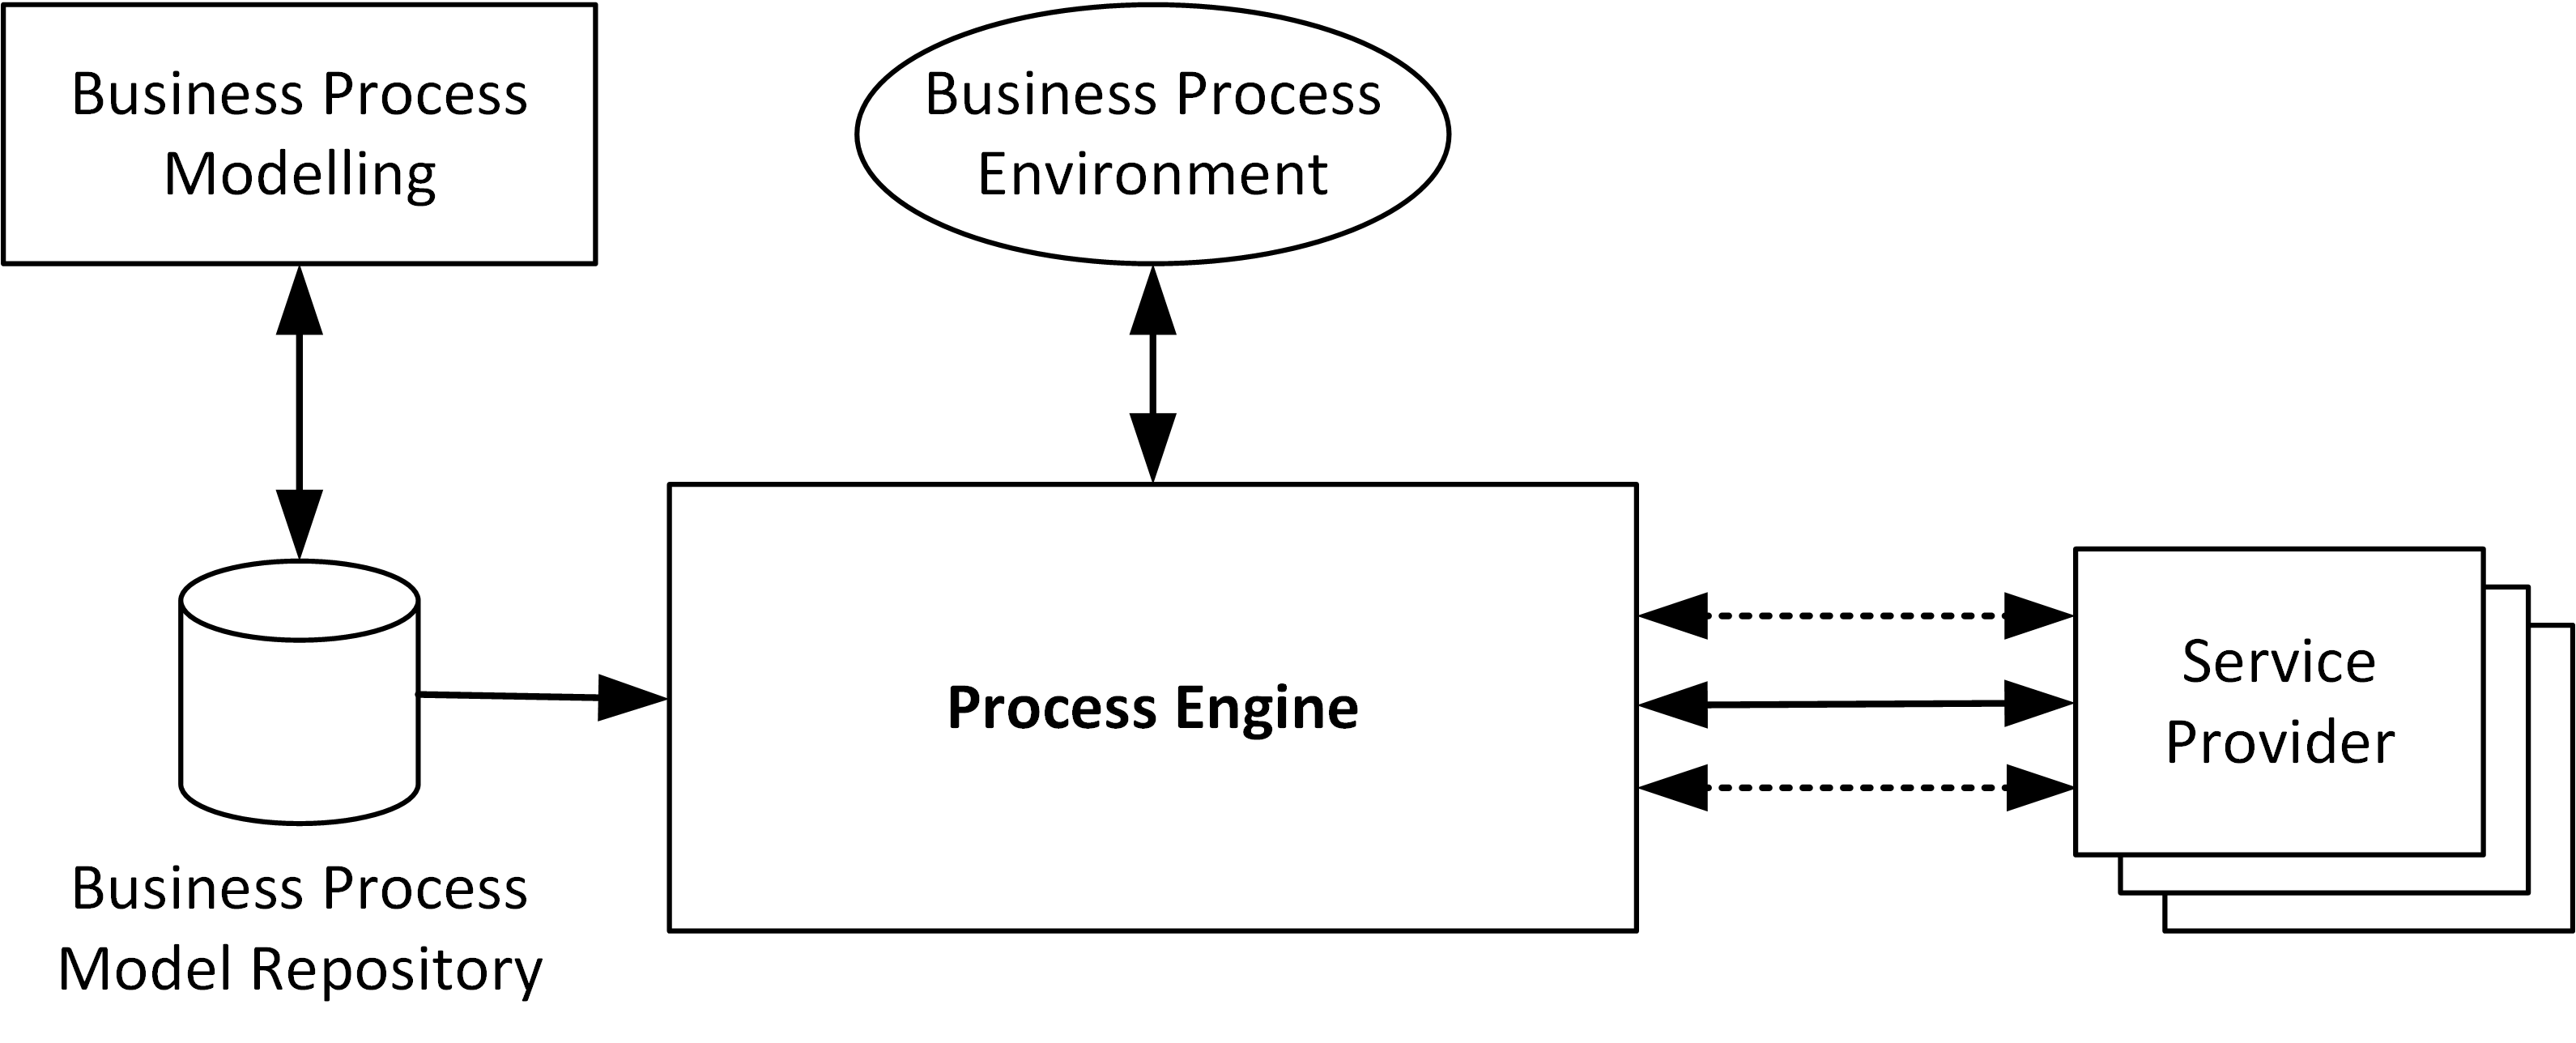
\includegraphics[width=1\linewidth]{chapters/background/bpm-architecture.png}}
	\caption{Business process management systems architecture model (see~\cite{weske:bpm-book},~p.~120)}
	\label{fig:bpm-architecture}
\end{figure}


\paragraph{The Camunda Business Process Engine}
A large, growing number of process engines is available on the market, including solutions from IT giants like SAP, IBM and Oracle.
In this work, \emph{Camunda BPM}~\cite{camunda} has been chosen to illustrate implementations.
As of August 2017, the software product is available in version 7.7.0 and comes in a commercial, regularly updated version and in a free, community-driven solution that is updated with every major release.
Camunda is popular among the research community as the source code is openly available, the product is mature, but actively developed and offers comprehensive support for BPMN 2.0. It is designed to be extensible and easily modifiable to adapt to custom requirements.
\emph{Camunda BPM} comprises a modeling tool, the Camunda process engine core and a number of browser-based user-interfaces to control process enactment and monitor execution state.
\autoref{ch:implementation} will provide further details about the engine architecture and extension mechanisms.


\subsection{Business Process Model and Notation}

A generic meta model of business process models is proposed in \cite{weske:bpm-book}.
According to the model, all processes are composed of nodes and edges with each node representing either an activity model, an event model or a gateway model. The complete definition is provided in \textit{Definition~3}.

\begin{description}
	\item[Definition 3 (Business Process Meta Model):]
	Let $C$ be a set of control flow constructs. $P = (N,E,type)$ is a \textit{process model} if it consists of a set $N$ of nodes, and a set $E$ of edges. \cite{weske:bpm-book},~p.~91
	\begin{itemize} 
		\item
		$N = N_{A}\cup N_{E}\cup N_{G}$, where $N_{A}$ is a set of activity models, $N_{E}$ is a set of event models and $N_{G}$ is a set of gateway models. These sets are mutually disjoint.
		\item 
		$E$ is a set of directed edges between nodes, such that $E\subseteq N \times N$, representing control flow.
		\item
		$type:N_{G}\rightarrow C$ assigns to each gateway model a control flow construct.
	\end{itemize}
\end{description}

Given the general semantics of business processes, a specific modeling notation has to be selected to express an informal process description in a formal, interchangeable way.
Different languages and notations have become available over the years, each serving different specializations.
Kossak~et~al.~\cite{kossak:bpmn2} organize some of the more popular languages as follows: A subset of them are focused on the control flow of business processes, for instance \ac{BPMN}~\cite{bpmnspec}, Yet Another Workflow Language and Petri Nets; some focus on object-orientation, like the \ac{UML} activity diagrams and use case diagrams; some are data-flow oriented, e.~g.~the Structured Analysis and Design Technique.
%\todo[inline]{references to the other languages}

Among these, the \acf{BPMN} has developed into a widely-adopted industry standard, also becoming ISO-standard in 2013~\cite{iso2013bpmn}.
The specification is developed by the Object Management Group~\cite{omghome} and now available in version 2.0~(January~2011) after being first released in January~2008. Whenever referring to BPMN in this work, version 2.0 of the standard is meant.
\acs{BPMN} can be understood as an extension to the abstract business process meta model adding a comprehensive catalog of visual representations and semantic constructs on top of a meta model. Furthermore, one of the most important features of its latest version is the a standardized interchange format provided through an \acs{XML} specification, as \cite{weske:bpm-book} points out.
As emphasized by \citeauthor{Muehlen:2007}~\cite{Muehlen:2007}, the increased expressiveness of modern languages like \acs{BPMN} comes at the cost of an increased complexity. An aspect that, apparently, did not stop it from gaining popularity.

\paragraph{Elements of a BPMN Model}
Following the abstract business process meta model, the core elements in any BPMN model are flow elements~(nodes) and connecting objects~(edges).
Flow elements can be either \textit{Events}, \textit{Activities} or \textit{Gateways}, each of them coming in different variations.
This section will introduce a subset of the elements available through the \acs{BPMN} specification to build the foundation to comprehend the thoughts presented in this work.

\begin{figure}[]
	\myfloatalign
	{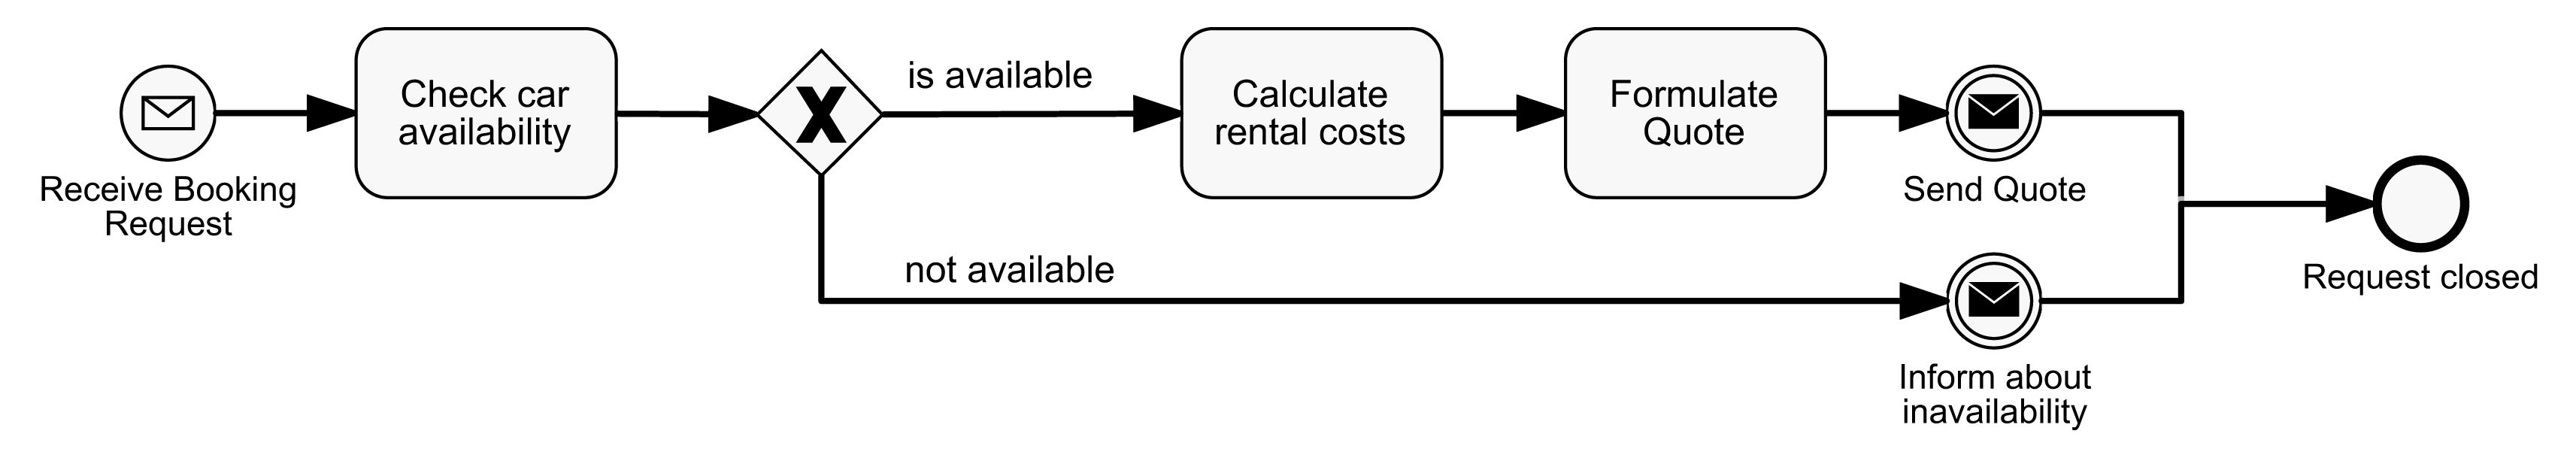
\includegraphics[width=1\linewidth]{chapters/background/intro-rental-car.png}}
	\caption{Simple BPMN model of issuing a quote for car rental}
	\label{fig:simple-bpmn-model}
\end{figure}

\autoref{fig:simple-bpmn-model} shows how a booking request might be handled in a car rental business.
Circular elements represent events, diamond-shaped elements are gateways. Activities are visualized by rectangles with rounded corners.
The given process gets instantiated whenever a booking request request is received from a customer, shown as a Message Start event. 
As a first step, the employee assigned to handle the request must check if the desired car is available. To that follows an exclusive OR-Gateway, distinguishing the further process flow depending on the availability of the car.
If the car is available, the quote must be created in two sequential tasks to be then sent out by the \textit{Send Message Event}. If the car is not available, the customer is informed about the closing of his request. 
In either case, the process ends with an \textit{End Event} after the customer was informed about the result of his request.

The example illustrates the basic use of activities, events and gateways in BPMN. However, for each type of element, activities, gateways and events, BPMN offers a variety of different kinds.
%Each of them comes in a broad variety.
The Task elements shown in the example~(\eg \,\textit{Check car availability}) are the most basic type of activities, representing \textit{a~unit of work}. The nature of a task can be further specified using task types, all activities can be additionally annotated with activity markers. Each of these modifications describes the activity semantics in a more detailed fashion.
Apart from the utilized XOR-gateway~(the execution-flow will proceed in exactly one of the outgoing branches), there is for example the parallel gateway, activating all outgoing branches. Moreover, the Event-based Gateway, which is followed only by events and continues along the branch of the first event that occurs.
Last but not least, message events are used to represent the action of sending information in the form of a message to a certain recipient. Other available event types are, for instance, timer, signal or error events. Events can occur as \textit{Start Events} (\eg \,\textit{Receive Booking Request}), where they trigger the instantiation of a process. Furthermore as intermediate events (\eg \,\textit{Send Quote}) or as end events, being fired when the process terminates. They can be \textit{catching}, \ie \,receiving a trigger, or \textit{throwing}.

Multiple participants taking part in a process can be expressed using \textit{pools}, which can be sub-divided into \textit{swimlanes}.
Interactions between different pools take place using message flows, which are depicted by a dashed arrow.
An example of such a \textit{Collaboration Diagram} is shown in \autoref{fig:bg:rental-car-customer}. It describes the previously discussed car rental process from the side of the customer, including the information exchange between rental company and customer.
When the airline issues the booking confirmation of the flight, the customer has to book a rental car and a hotel. The hotel booking is modeled using a collapsed sub-process to reduce the complexity of the model.
After issuing the rental car request, an event-based gateway shows that the process is ready to consume any one of the two event messages. If the booking was successful, the control flow proceeds to the inclusive join gateway and the process can terminate once the hotel booking is also completed. If the car rental company informs about unavailability, the customer starts looking for an alternative car option.
A data object is used to model the \textit{Request} artifact as output of the \textit{Prepare~Request} task and as input to the message throw event.

\begin{figure}[]
	\myfloatalign
	{\hspace*{-0.8cm}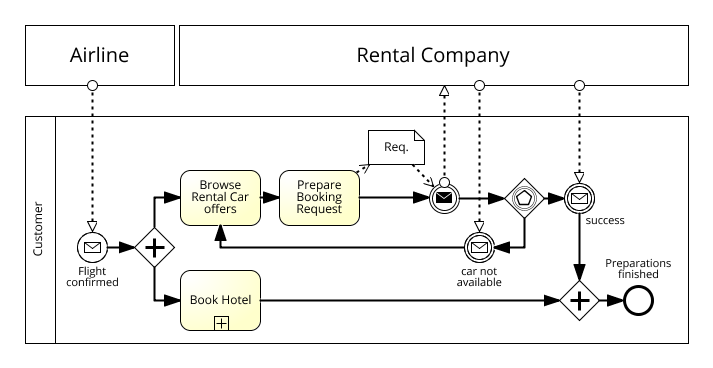
\includegraphics[width=1.1\linewidth]{chapters/background/intro-rental-car-customer.png}}
	\caption{Rental car booking process with multiple participants}
	\label{fig:bg:rental-car-customer}
\end{figure}


\section{Complex Event Processing}\label{ch:bg:cep}
The IT world is facing an exponential increase in the amount of produced data. A significant part of this data are pieces of information about real-life occurrences, such as a current sensor value, an interaction on a website or the location of a vehicle on the road.
We call this kind of strongly time-related information an \textit{Event} and the according computer science field \acf{CEP}~\cite{evtprocessing}.
More specifically, Etzion and Niblett define an event as \textit{an occurrence within a particular system or domain; it is something that has happened, or is contemplated as having happened in that domain}.
It is understood that events are of a certain \textit{event type}, defining the attributes that each event instance of the event type is composed of. An attribute is described by a unique attribute name and a data type.

\begin{description}
	\item[Definition 4 (Event):]
	An event is a tuple $e = (et, eventtime, c)$, whereas
	\begin{itemize} 
		\item
		$et$ is the event type
		\item 
		$eventtime$ is the time the event happened
		\item
		$c$ is the content of the event consisting of a set of key-value-pairs according to the content description cd of the corresponding event type $et$.
	\end{itemize}
\end{description}

%An event processing network is a collection of event processing agents, producers, consumers, and global state elements, connected by a collection of channels

Four major components take part in an event processing network: (a) An \textit{event producer} provides information to the system, (b) an \textit{event agent} processes the occurring information, so that it can be delivered to the \textit{event consumer}~(c). The components are linked through \textit{event channels}~(d).
Typically, a so-called \textit{\acs{CEP} Engine}~(also: CEP platform) is at the heart of the system, taking the role of an event agent.
Modern CEP platforms are trimmed to maximum efficiency, being able to process hundreds of thousands of events every minute.
Their main purpose is to accept incoming events from event producers, filter and match them according to selection criteria and, finally, derive a new event occurrence to be sent to the registered event consumers.

% cite luckham2008power

\paragraph{The publish/subscribe Principle}
In event-based architectures, communication takes place according to the \textit{Publish/Subscribe Principle}.
The concept essentially demands that an event processing middleware publishes events to processes only after they have issued a subscription for these events.
Consequently, there is a strict temporal order between the actions subscribe, consume and un-subscribe(\autoref{fig:bg:pubsub-workflow-temporal-order}). The consumption and un-subscription can only happen after the subscription. Once an un-subscription has been issued, no consumption can follow.~\cite{tanenbaum:2007}

% mandal also references Barros, A., Decker, G., Grosskopf, A.: Complex events in business processes. In: Business Information Systems. Springer (2007)

\begin{figure}[]
	\myfloatalign
	{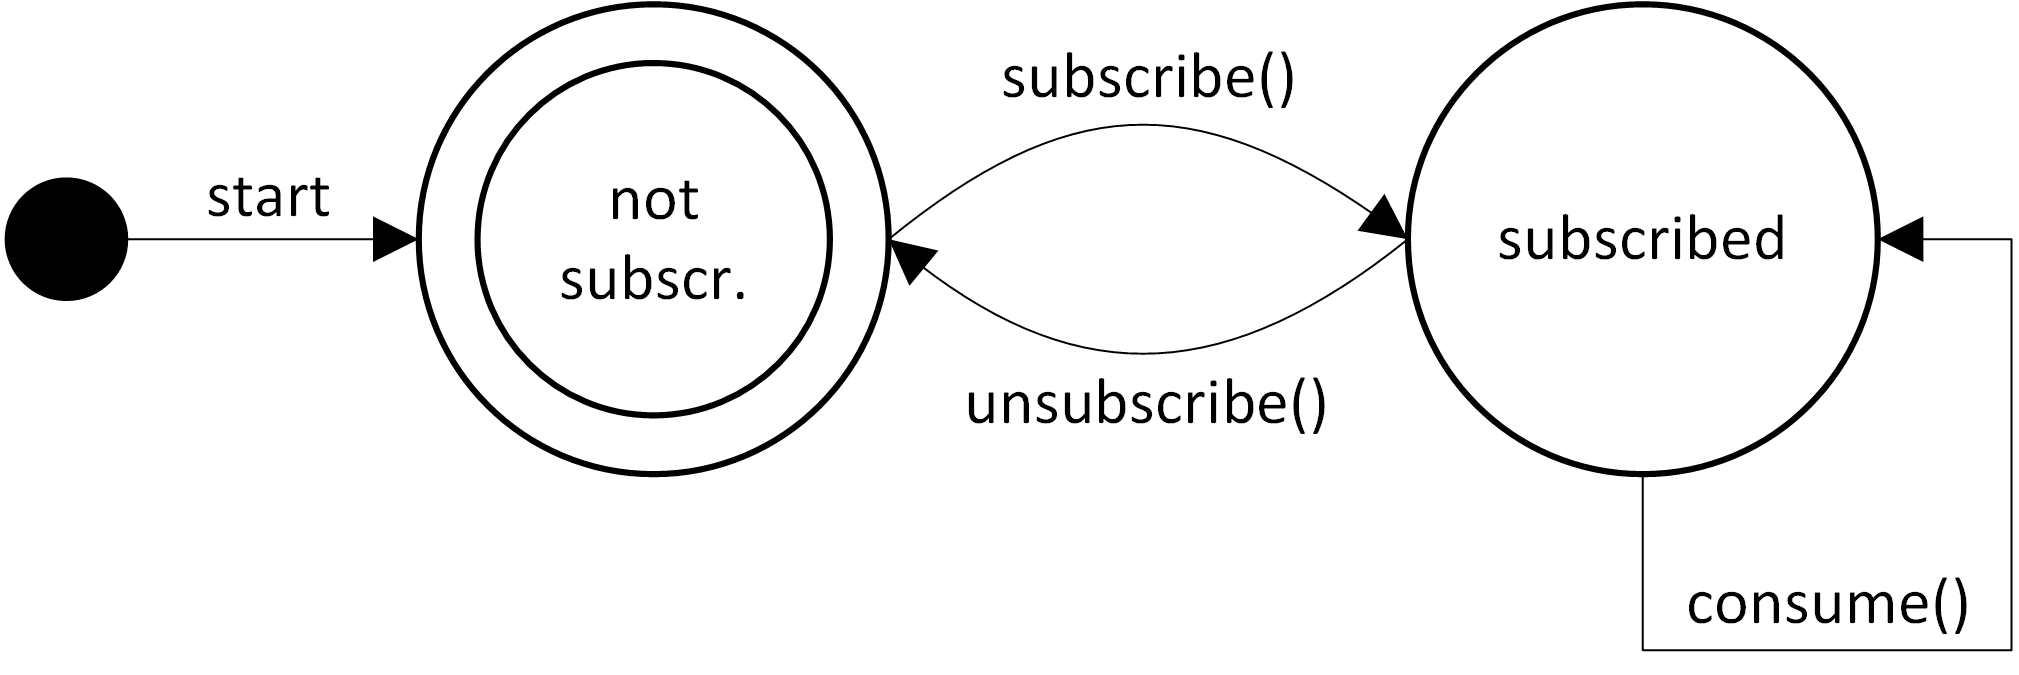
\includegraphics[width=0.6\linewidth]{chapters/background/pub-sub-statemachine.png}}
	\caption{Publish-Subscribe workflow expressed in a state diagram}
	\label{fig:bg:pubsub-workflow-temporal-order}
\end{figure}


One of the main advantages of this principle is, that the involved parties are \textit{referentially decoupled}. They do not need to explicitly refer to each other, an aspect that is also acknowledged in~\cite{evtprocessing}.
Their decoupled nature facilitates the management and development of event processing networks. Event producers and consumers might change frequently.
Whenever a new event source is available it can be connected to the CEP platform without considering all future consumers. Consumers can subscribe and un-subscribe without influencing the operations on the consumer side.


\paragraph{Stream Processing}
To be able to cope with potentially large amounts of data, Complex Event Processing Platforms work on the basis of \textit{stream processing}.
In a traditional relational database, information is stored for an indefinite amount of time. When a user queries the data store, the system processes the tabular data and calculates the requested result. 
The advantage of this approach is that the user can access historic data at any time, as long as it is not explicitly deleted from the database.
In many occasions, the amount of available data significantly surpasses the storage capacities and that concept can no longer be followed.

Stream processing addresses the mentioned challenge by largely reducing the amount of data that is persisted in the system. Instead, it is the goal to keep only those pieces of information, that are necessary to process a result for currently registered queries.
Incoming data objects, or events in the case of a CEP platform, enter the event stream and are immediately evaluated against all existing query expressions. If the information is not required to process any of the queries, it is deleted instantly. If an event matches a query, a notification is sent to the subscribed consumers. \autoref{fig:bg:stream-processing} illustrates the concept.
As a consequence, a certain event can not be part of a query result, if that query has been registered after the occurrence of the event.
In case aggregated information is demanded by the query, the stream processor will internally store aggregated information, but not keep every information that led to the aggregated value.~\cite{streamprocessing} 

\begin{figure}[]
	\myfloatalign
	{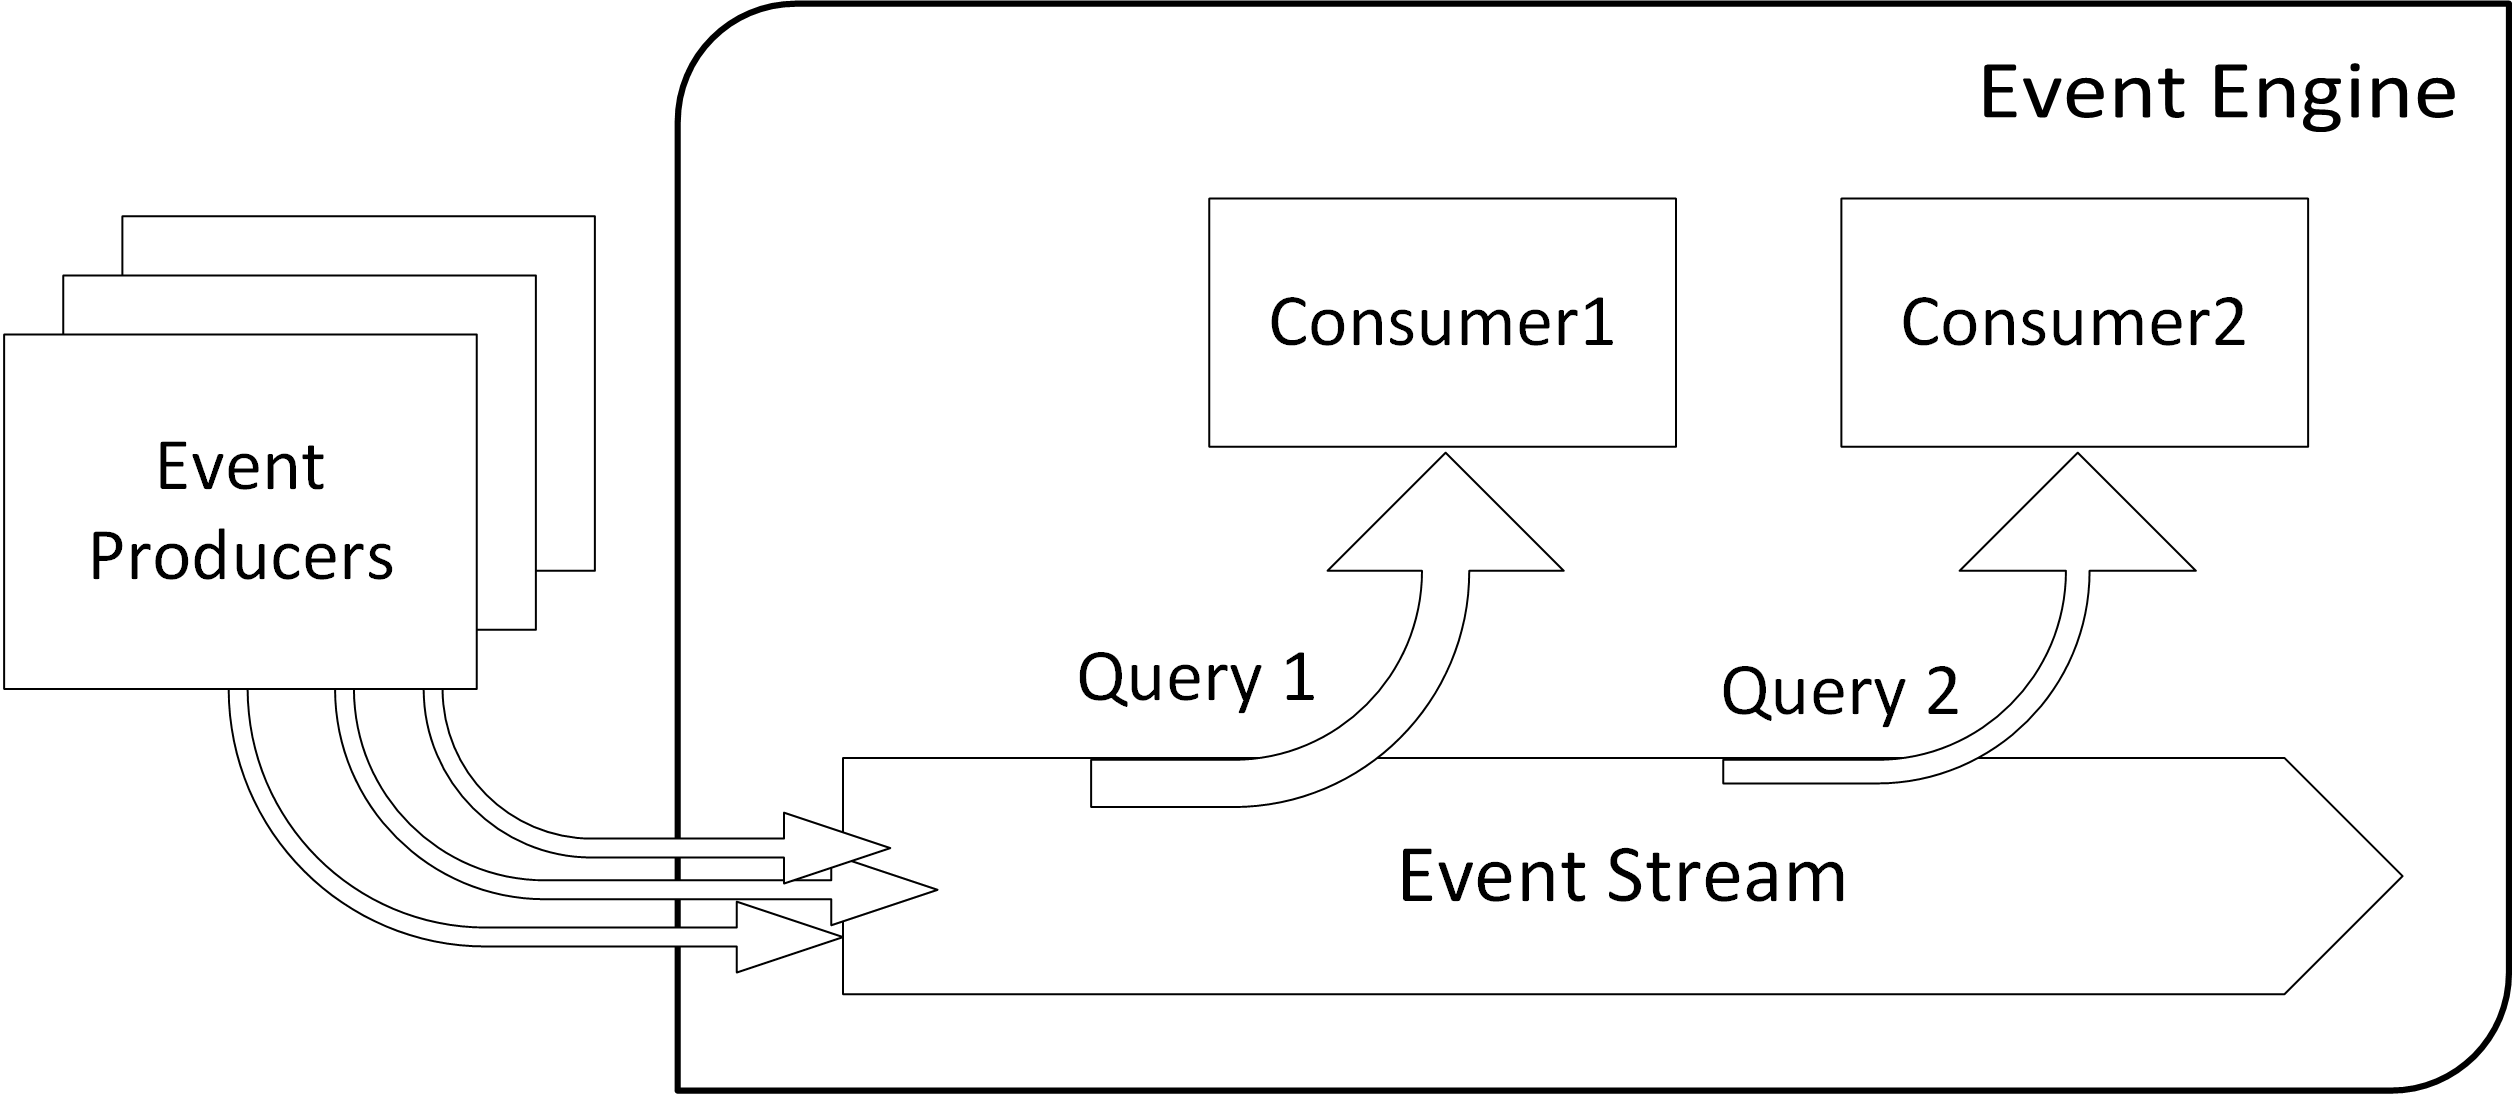
\includegraphics[width=0.7\linewidth]{chapters/background/cep-stream-processing.png}}
	\caption{Stream processing concept applied in a CEP Engine}
	\label{fig:bg:stream-processing}
\end{figure}

The subscription to an event in a CEP platform is primarily defined by an \textit{Event Query}.
Many modern event query languages are inspired by \acs{SQL}, but cannot be entirely compliant due to the different underlying data processing concept.
When formulating event queries, it is essential to consider the stream processing principle.
For the illustration of the concepts, this thesis relies on the Esper \ac{EPL}~\cite{esperhome}, utilized in Esper-based event processing engines like the one employed in the presented reference implementation, \autoref{ch:implementation}.
A simple event query in Esper looks as follows:

\begin{lstlisting}[language=sql,caption={Sample Query in Esper EPL},label=lst:epl-query-example]
	SELECT occurrencetime, delay, delayreason 
	FROM eurotunnel.win:time(2 hour)
	WHERE delay > 30
\end{lstlisting}

\section{Event-driven Business Process Control}
The disciplines of Complex Event Processing and Business Process Management are connected in \acf{EdBPM}, which discusses the uses of events to enhance business processes~\cite{evtprocessing}.
There are two usage scenarios for events in BPM. In Business Activity Monitoring and analysis, events are published by the process engine and processed to obtain analytical information, for instance about process status, efficiency or errors.
This thesis considers events from the second perspective, \acf{EdBPC}. The field focuses on the business process as an event consumer.
Within business processes, event-based communication can for example be used to exchange information between participants or to react to external events. While the BPMN supports a large variety of different events, we are going to investigate message events specifically. Whenever talking of an event-occurrence, it can be assumed that the term \textit{event} implicitly refers to a message-event in the BPMN context.

\ac{EdBPC} using external event sources is facilitated by connecting the business process engine to an event engine.
As explained in \autoref{ch:bg:cep}, interactions with a CEP platform follow the publish-subscribe paradigm.
In the BPM scenario, this means that a subscription to events must be present, so that events can be received by the process engine and correlated to a specific message element within a process instance~\cite{Baumgrass2016}.
The correlation has to be performed by the process engine on the basis of context information, for example a subscription identifier incorporated inside every CEP message. 
An interaction between process engine and event engine is illustrated in \autoref{fig:bg:subscription-workflow}~\cite[,\,p.\,13]{mandal:2017} at the example of the event engine Unicorn.
Note that a different event engine might implement the work-flow slightly differently, but still follow the same general concept.
In the given case, the process engine first issues a \acs{HTTP} POST call containing the subscription query a notification-path. The path contains the address of the desired notification recipient in case a matching event occurs.
The event engine answers that call with a unique identifier associated to that single subscription.
As soon as an event occurs that matches the query, the event engine sends the query output along with the subscription identifier to the process engine which can correlate the event back to the associated instance.
In the next chapter, we will discuss when exactly the event subscription is issued by the process engine.

\begin{figure}[]
	\myfloatalign
	{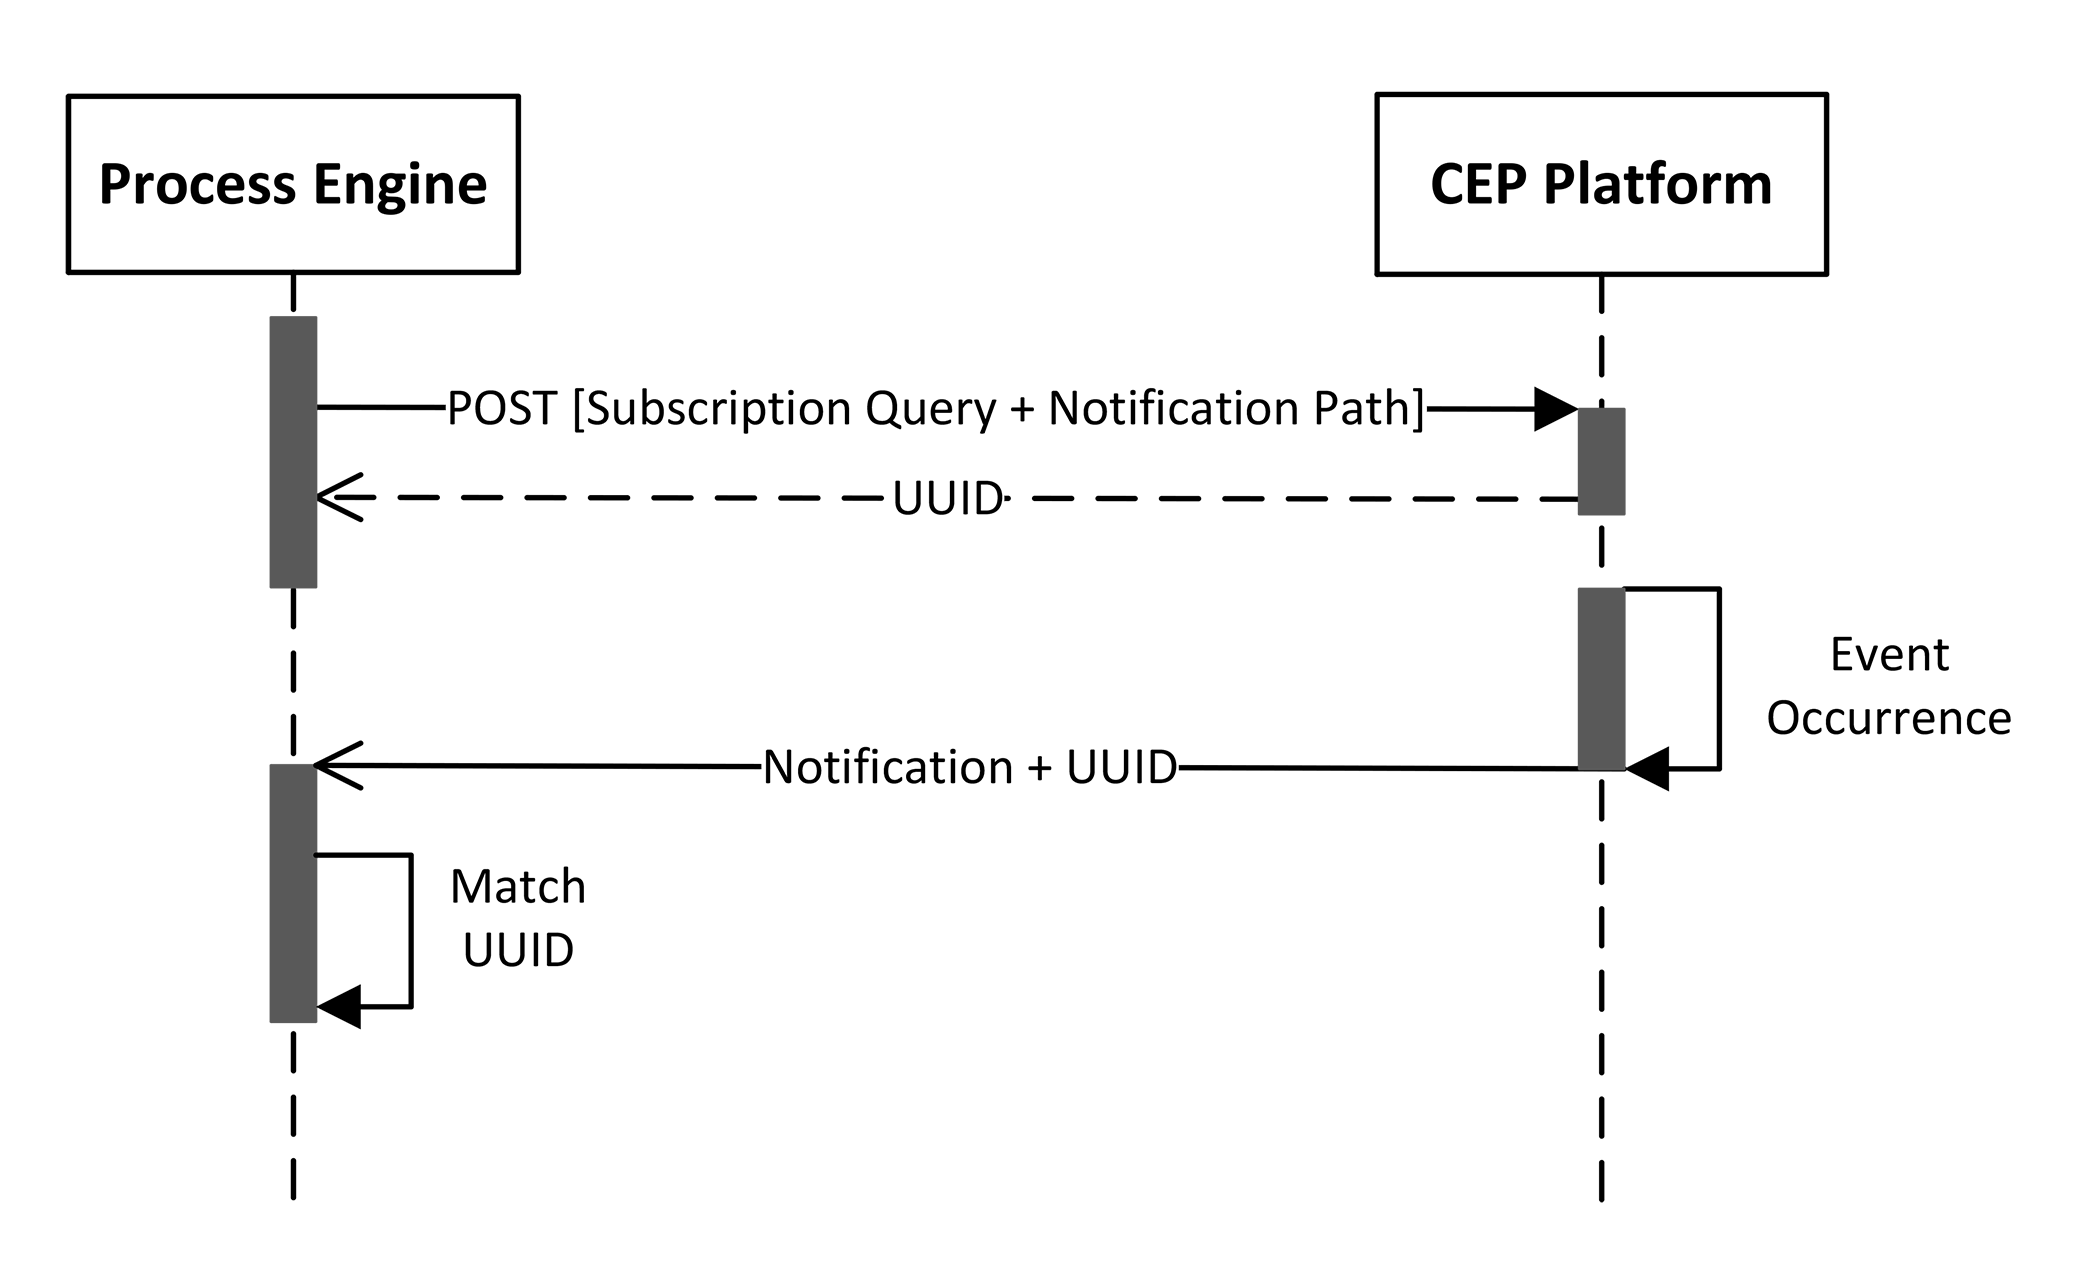
\includegraphics[width=0.6\linewidth]{chapters/background/subscription-workflow.png}}
	\caption{Even-subscription work-flow between process engine and event engine.}
	\label{fig:bg:subscription-workflow}
\end{figure}

%- no standard yet available to do subscription in bpmn
%- it must be assumed that the subscription is either already active or explicitly modeled in BPMN, e.g. using a service task
%- OR given the BPMN spec it is generally assumed that the subscription is executed as soon as en event is enabled
%- further analysis of this topic is provided in ...
%- the time of event subscription is clear for start events
%- Correlating events to process instances






%\addtocontents{toc}{\protect\clearpage} % <--- just debug stuff, ignore
%************************************************
\chapter{Problem Statement}\label{ch:problemstatement}
%************************************************

Event subscription is an essential part of event-driven architectures and must consequently be considered when using events in business processes.
While the use of external events is an active topic in research, most approaches only briefly discuss the subscription mechanism and use the \acs{BPMN}~semantics for orientation~(\eg \,\cite{Pufahl2017} and \cite{Baumgrass2016}).
Though event subscription is not directly addressed in the BPMN~specification, the descriptions on intermediate events state:

\medskip
\textit{"For Intermediate Events, the handling consists of waiting for the Event to occur. Waiting starts when the
Intermediate Event is reached. Once the Event occurs, it is consumed."}~\cite{bpmnspec},~p.~440

\medskip \noindent The usual interpretation of this excerpt is that the subscription to the event takes place as soon as the event gets enabled, the un-subscription when the event terminates.
As pointed out by Mandal~et.~al.~\cite{mandal:2017}, these subscription semantics significantly limit the flexibility of using events in business processes and can cause undesired behavior and fault.
Due to the strict temporal order between event subscription, occurrence and un-subscription as required by the publish-subscribe paradigm, any events that occur before the enabling of the event element will be ignored by the process execution.
That reduces the timespan for events to occur to a potentially small part of the total execution time and means that crucial events might be missed which can delay or block a process execution unnecessarily.

In the following section, the problem is further illustrated at the example of two motivating scenarios.
The observed situations then lead to the definition of \textit{Event Occurrence Scenarios} and the derivation of a set of requirements that must be fulfilled by a mechanism for flexible event subscription in business processes.

\section{Motivating Examples}\label{ch:motivatingexamples}
% some has been mentioned in the introduction
%illustrate the complexity

To allow a better understanding of the issue, event-driven use-cases from two different domains are presented in the following.
The cases are revealed through their standard BPMN representation.
It is illustrated, why the time of event subscription is of great importance which motivates to study the mechanics and implications of event subscription in business processes.

\paragraph{Delay of a logistics process}
The first example~(\autoref{fig:example-eurotunnel}) is taken from the logistics domain and shows a truck transport that has to cross the English Channel.
The truck driver receives the transport plan for his next tour from France to the UK. By default, the company crosses the Channel using the Eurotunnel, an underground train connection between London and Paris.

\begin{figure}[]
	\myfloatalign
	{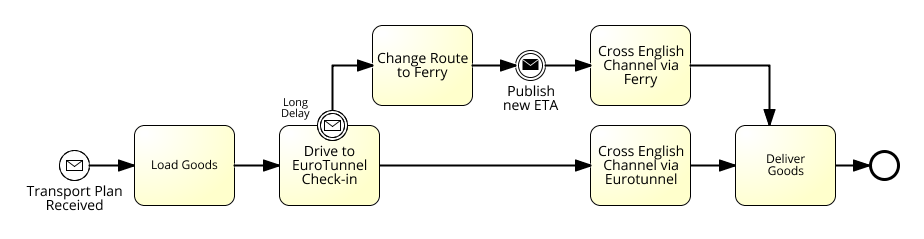
\includegraphics[width=1\linewidth]{chapters/requirements/Eurotunnel-simplified.png}}
	\caption{BPMN Model of a Logistics Process using events for route~optimization~(Example 1.1)}
	\label{fig:example-eurotunnel}
\end{figure}

After loading the goods at the factory, the truck will head towards the check-in location of the Eurotunnel.
If everything runs on schedule, the truck crosses the channel on the train and then delivers the goods in Great Britain.
Alternatively, the process considers a route using the ferry from Calais~(FR) to Dover~(UK).
The Eurotunnel administration publishes delay information approximately every 30~minutes through an RSS feed on their website. While it mostly operates on schedule, delays ranging from 15~minutes to several hours occur regularly. It can happen that new information is not published for multiple hours.
Significant delay events (delay~>~30~minutes) are received through a boundary catching message event attached to the activity \textit{Drive to Eurotunnel Check-In}. The boundary event is interrupting, hence the activity is canceled if a delay occurs.
The transport continues towards the ferry terminal and crosses the English Channel over sea. After crossing the channel, the goods are delivered to the recipient.

As interpreted from the BPMN specification, the subscription to the boundary event is issued as soon as the related activity is enabled.
Given that events arrive every 30~minutes, there can be a gap of up to half an hour, before the first information becomes available.
In the worst cases, when data isn't published for several hours, this gap will be even bigger.
Let's consider a very busy weekday; A technical fault occurred in the tunnel earlier that day and the train runs 3 hours behind schedule.
The last information on the RSS feed was published at 2:35\,pm. At that time the truck driver is still in the process of loading goods, finishing the activity at 2:40\,pm.
Following the process definition, the driver now departs towards the Eurotunnel check-in.
The system publishes updated information at 3:15~pm, operations are still 2:30\,h behind schedule. The message gets received through the process and the truck driver takes the alternative route to the ferry, but only after heading to the Eurotunnel for 35~minutes. The late change of plans causes an unnecessary delay to the shipment.

\begin{figure}[]
	\myfloatalign
	{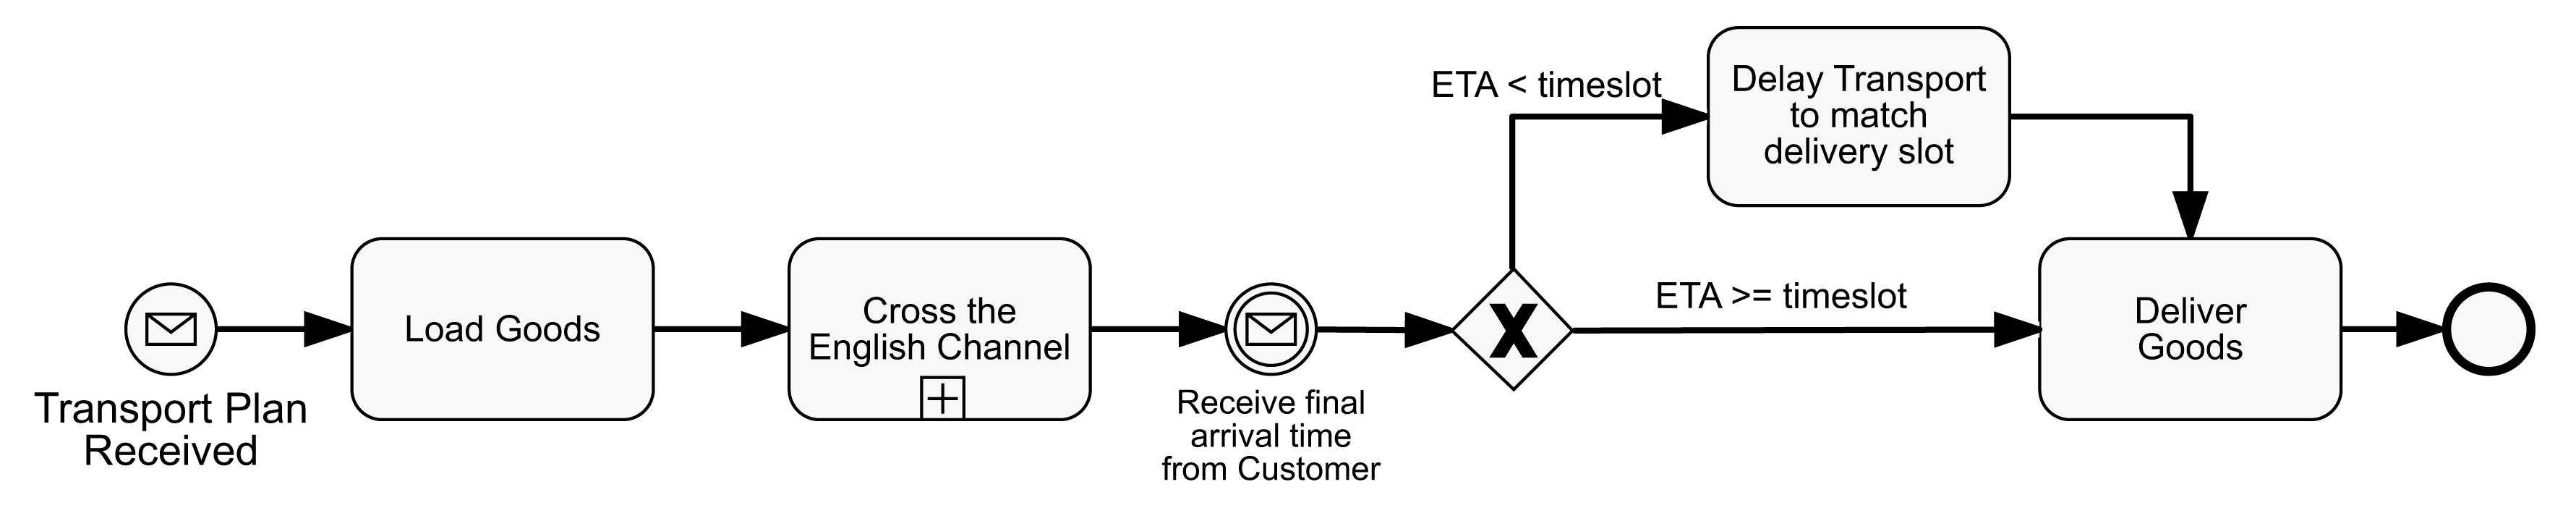
\includegraphics[width=1\linewidth]{chapters/requirements/Eurotunnel_part2.png}}
	\caption{Transport via English Channel that is timed to a delivery~slot~(Example~1.2)}
	\label{fig:example-eurotunnel-part2}
\end{figure}

\autoref{fig:example-eurotunnel-part2} is an extension of the the transport process.
In logistics, it is common that a delivery cannot be accepted at an arbitrary time. Instead, the receiving party assigns delivery windows to the transport company.
The transport must arrive during the given time window, otherwise the delivery cannot be completed.
After crossing the English Channel, the process model shows the catching of a message event containing the desired final arrival time at the factory. There is an agreement with the factory, that the delivery slots will be approved 2~hours before the expected arrival.
If the current ETA of the transport is greater or equal to the arrival time, the driver will head to the drop-off point immediately. If the transport is ahead of schedule, the driver will have to delay the delivery to match the time window.

The presented process model illustrates another complexity of using events in processes. Again, the listening to the announcement of a delivery window will start when the event element is enabled, in this case after crossing the English Channel. 
Until an event has been received, the process will not continue. 
Much worse: if the receiving party sends out the arrival time information too early, \ie~while the truck is crossing the channel, the event is missed. If it is not issued again, the process cannot receive a message and will get stuck indefinitely waiting to catch the event.

Neither of the two presented catch events allow for an efficient and reliable execution of the process. They can cause unnecessary delays and even blocking of the process execution.


\paragraph{Up-to-date shipping information for an order}
\begin{figure}[]
	\myfloatalign
	{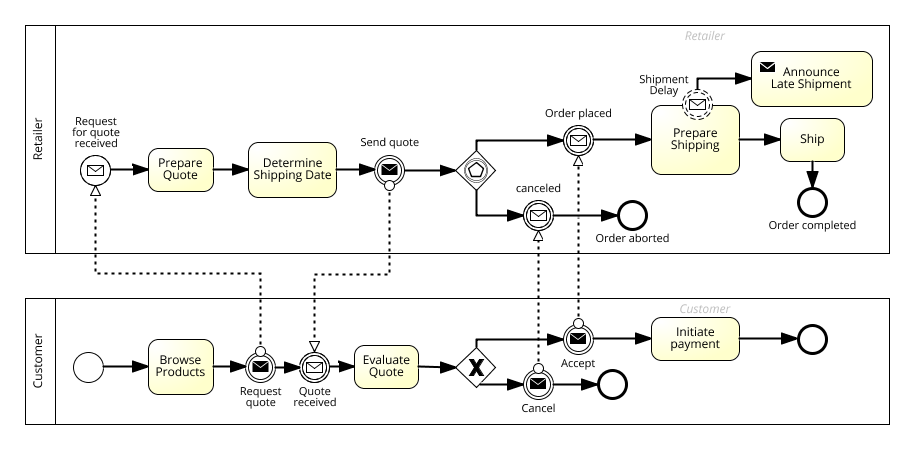
\includegraphics[width=1\linewidth]{chapters/requirements/Retail-Order.png}}
	\caption{Model of a retail order management process (Example 2)}
	\label{fig:example-order}
\end{figure}

A~similar situation can be observed in the order-management process depicted in \autoref{fig:example-order}.
It describes the interaction between customer and seller in a traditional distance retail scenario: After browsing the product catalog, the customer requests a quote for the articles he or she is willing to buy.
The retailer makes an offer including an approximation of the expected shipment date and sends it to the customer. That quote is then either accepted or not and the payment is issued if necessary.
Once the retailer is informed about the placement of the order, the products are packed and shipped as soon as possible.
For articles that are not currently in stock, the retailer must await the shipment from the factory. If any of the factory-shipments is delayed, the retailer cannot ship in time and will announce a delayed shipment date to the customer.
This situation is modeled through a non-interrupting boundary event attached to the \textit{Prepare Shipping} activity, which triggers the sending of the updated shipment date to the customer.

The process shows a number of similarities, but also differences in terms of event-use when compared to the logistics process in Example~1.
At first we look at the three intermediate catch events, \textit{Quote~received}, \textit{Order~canceled} and \textit{Order~placed}.
In each of the cases, the event to be caught is the direct response to a message that was sent right before. While the process will also enter a waiting state until the response arrives, that waiting is not to be interpreted as an unnecessary delay to the process execution.
Other than in Example~1.2\,(\autoref{fig:example-eurotunnel-part2}), there is nothing useful to do before the response is received.
It is furthermore worth noting that the response messages cannot be missed, because the message catch event immediately follows the message send event.

A different situation holds for the boundary event \textit{Shipment Delay}.
While the subscription to a Eurotunnel event can be issued at any time, it does not depend on any process data, the shipment delay has to be observed for each product that is part of the order. A subscription can therefor not be executed before the activity \textit{Prepare~Quote} has terminated.
The Esper query to obtain delay information about the product with the id 123 looks as follows:

\begin{lstlisting}[language=sql,caption={Esper EPL Query to obtain delay information for a product},label=lst:epl-query-shipping-delay]
SELECT newArrivalDate, delayAmount, delayReason, productId
FROM shippingdelay
WHERE productId = 123
\end{lstlisting}

\noindent Conforming to the definition of the process, the system will listen to shipment delays once the activity \textit{Prepare~Shipping} is enabled and therefor much later than possible.
Any events that occur after the completion of \textit{Prepare~Quote} but before \textit{Prepare~Shipping}, cannot be considered in the process execution and the customer will not be informed about a possible late shipment. That will, for instance, concern events that occur while the customer makes the decision about accepting or canceling the order.

% The first of these three follows the \textit{Send/Receive} Service Interaction Pattern. \todo[inline]{missingref}
% Two parties interact 

\medskip \noindent 
The two presented examples have illustrated the complexity of using events in business processes, especially when all possible event occurrence times are taken into consideration.
Differences have been pointed out as to how exactly the event is placed in the process, if it waits for a direct response to an earlier request or if the event occurrence is unrelated to the execution of that very process.
Motivated by this complexity and the possible implications, it is the goal of this work to evaluate the capabilities of BPMN and to present a concept for the flexible handling of event subscription in business processes.


\section{Event Occurrence Scenarios and Time of Subscription}\label{ch:ps:eos}
Given the motivating examples, a generic set of \textit{Event Occurrence Scenarios} is defined in this section. 
Each of the scenarios represents a real-world situation and process implementations need to be capable of handling them to avoid negative effects.

\medskip \noindent
The dominant variable to consider is the event occurrence time.
According to the BPMN specification, it is possible to catch an event if it occurs after the event element is enabled. As shown before, it is often impossible to control occurrence time and events do occur outside of the listening time intervals.
An \ac{EOS} describes the time of event occurrence in relation to a specific step in process or engine execution.
The life-cycle of a process within a process engine is explained in \autoref{ch:bg:bpm} and taken as reference. It is assumed that the process and event engine are configured and running.
An event is considered to always occur before or after a life-cycle step or in between two consecutive steps. 
Given the life cycle steps \textit{process deployment}, \textit{process instantiation} and \textit{event enabling}, the following occurrence scenarios are distinguished in this work:
% they have an implicit temporal order

\begin{aenumerate}
	\item[$EOS_{1}$] While the BPMN event element is enabled
	\item[$EOS_{2}$] The event does not occur
	\item[$EOS_{3}$] Between process instantiation and \\the enabling of the BPMN event
	\item[$EOS_{4}$] Between process deployment and \\process instantiation
	\item[$EOS_{5}$] Before process deployment
\end{aenumerate}\label{def:occurrence-times}
% they are ordered this way to be in line with the assessment chapter

\begin{figure}[]
	\myfloatalign
	{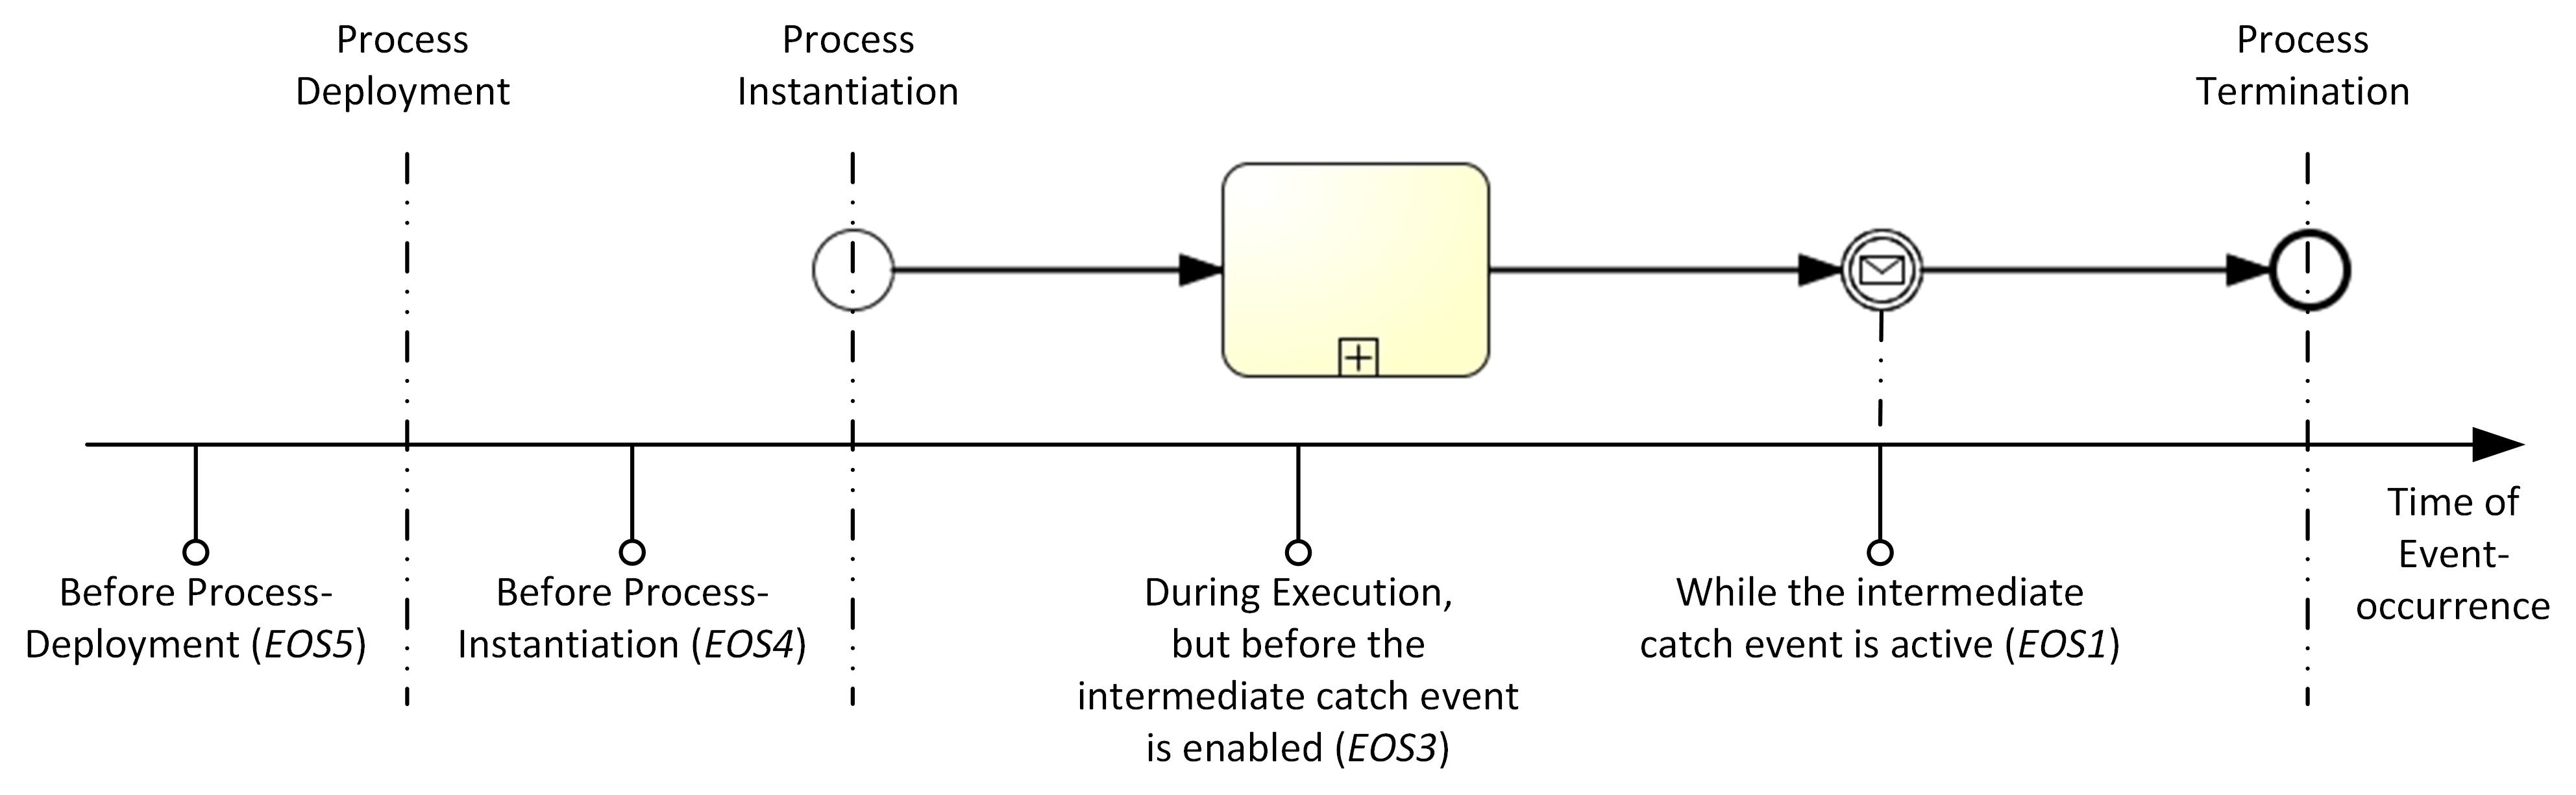
\includegraphics[width=1\linewidth]{chapters/requirements/timeline_event-occurrence.png}}
	\caption{Event Occurrence Scenarios}{Possible times of event occurrence in relation to a process execution life-cycle. \textit{EOS2} (event does not occur) not illustrated.}
	\label{fig:occurrence-timeline}
\end{figure}

\noindent An overview of the EOSs and the related life-cycle steps is provided in \autoref{fig:occurrence-timeline}, which uses a time-line to illustrate the possible event occurrence times.
The model deliberately excludes event occurrences after termination of the event element, because that would presume that there is no more interest in the event as the execution flow continued on another branch. Otherwise, the process will remain in waiting state until the event occurs.

As introduced in \autoref{ch:bg:cep}, there is a strict temporal order between event subscription, consumption and un-subscription.
To catch an event that occurs as described in any of the EOSs, the related subscription operation has to be executed before the start of the time interval associated with the EOS.
On that basis, the latest possible event subscription time can be derived from each event occurrence scenario and is as follows:
\textit{before process deployment}~($EOS_{5}$), \textit{during process deployment}~($EOS_{4}$), \textit{at process instantiation}~($EOS_{3}$) and when the \textit{BPMN event element is enabled}~($EOS_{1}$).

It is important to highlight that the subscription to an event source can depend on additional context information or process data, which can be a significant limitation to the possible subscription time.
That situation is illustrated in \textit{Example~2}~(\autoref{fig:example-order}), where the subscription to the shipment delay information cannot be executed before the \textit{Prepare~Quote} activity is completed.
More generally put, a \textit{subscription~dependency} is defined as follows:

\begin{description}
	\item[Subscription Dependency]
	The subscription operation is \textit{dependent}, if any of its parameters, for instance the event query, contains a variable value that has to be determined at the time of subscription.
	The value might reference a piece of information from the process instance context, an engine-wide piece of data or external information.
	In case of a dependence, the subscription cannot be issued before the associated information is available.
\end{description}

If a subscription dependency resolves before the process execution reaches the event element, it should still be possible to flexibly chose the subscription time in the process.
For that reason, in addition to the four subscription-time options presented earlier, an additional option \textit{at any time during process execution} must be available.


\section{Requirements Definition}\label{ch:requirements}
The previous sections have exemplified how the BPMN execution semantics and notation capabilities limit users when using events in business processes. 
Now, these deficiencies are formalized into an initial set of requirements additional to the features offered by BPMN.
They build the foundation for enhancing BPM solutions towards flexible event subscription management~(\autoref{ch:flexibleeventsubscription}).
Before that, the formal requirements will be used to evaluate the capabilities of current Process Management Solutions~(\autoref{ch:assessment}), which results in an additional set of shortcomings \textit{S1} to \textit{S3} of current solutions presented in \autoref{ch:ass:discussion}.

%\medskip \noindent
%It shall be noted that the requirements \textit{R2.2} and \textit{R3} introduced in this chapter have also been pointed out by Mandal~et.\,al. in their work on early subscription and event buffering\,\cite{mandal:2017}.
%Note that the need for flexible event subscription has also been pointed out by Mandal~et.\,al. in their work on early subscription and event buffering\,\cite{mandal:2017}. The authors follow a similar line of argumentation and also specify the requirement for a flexible time of subscription and event buffering.


\paragraph{R1: Subscription Fundamentals}

\begin{description}
	\item[R1.1 Subscription to an Event Source:]
	To enable the reception of events from a publish/subscribe event source, the subscription operation must be part of the execution flow. 
	In accordance with the obligatory temporal order of operations, the subscribe operation must happen before an event can be received and/or the un-subscription takes place.
	\item[R1.2 Un-subscription:]
	As soon as events from the source must not be received anymore, an un-subscription has to take place.
	\item[R1.3 Availability of Information:]
	For each event that is used in a business process, all information necessary to execute an event subscription in the given execution environment must be available.
	That information generally includes the event query, the address of an event processing platform and auxiliary information to establish the communication, for instance authentication data.
	%While the event query is associated to a specific event element and must therefor be part of the process model, the process platform information might be valid for potentially all processes and can be made available through a global data store.
	\item[R1.4 Variables in Event Queries] 
	To adapt an event subscription to execution- or time-specific information, variables can be utilized as part of the query string.
	At the time of event subscription, these variables must be replaced their current values before the subscription is executed.
	
\end{description}

\paragraph{R2: Event Subscription Time}

\begin{description}
	\item[R2.1 Explicitness:] 
	For each event that is used in a business process, it must be possible to derive the time of event subscription from the process model. The time of subscription may either be explicitly stated or defined implicitly.
	\item[R2.2 Flexibility:] 
	The time of subscription can be influenced independently from the place the event element takes in the model. Timing options are made available to catch events according to any of the event occurrence scenarios EOS1, EOS3, EOS4 and EOS5. 
	Consequently, the options must include but are not limited to the subscription before process deployment, during  pr. deployment, at process instantiation, subscription at an arbitrary but explicit time during process execution or when the event element is enabled.
	Thereby, also events that occur after the time of subscription, but before the event element is enabled shall be available to be consumed.~(cf.\,\cite{mandal:2017})
	%By that means, the variability of the time of event occurrence can be specifically addressed in the process model and unnecessary delay or blocking of the execution can be reduced.
	\item[R2.3 Awareness of Subscription Dependencies:]
	The additional flexibility provided through \textit{R2.2} is limited by the use of variables in event queries~(\textit{R1.3}) and the implicit dependencies on context information.
	The execution environment must only allow a subscription time after the resolving of all dependencies.
	
	Dependencies can exist within a certain process instance, for example when an information from a local DataObject is referenced in a query. In more complex scenarios, the subscription might depend on data from other process instances or even other processes which must first be obtained.
\end{description}


\paragraph{R3: Event Buffering}

\begin{description}
	\item[R3.1 Buffering Principle:]
	%To make all events since the subscription time available during process execution, matching events need to be stored temporarily.
	As introduced by \textit{R2.2}, an indefinite time can pass between the time of subscription and the consumption of the event.
	While the subscription operation generally assures that the event is received, it is necessary to temporarily store it until the consuming element is reached.
	
	This temporary storage is referred to as an \textit{Event~Buffer}.
	The storage must be designed to fulfill the semantics demanded by \textit{R2.2} which means that any event that occurs after the time of event subscription must be available to consume.
	
	\item[R3.2 Buffer Scope:]
	The flexible event subscription time~(\textit{R2.2}) allows an event subscription after process instantiation, but also before process instantiation or deployment.
	It can be inferred that an event buffer operates either in the scope of a process instance, a process definition, or in the scope of the complete execution environment.
	To implement all event subscription times stated in \textit{R2.2}, the execution environment must support event buffering in each of the three scopes. 
	The provided concept must make clear to the user, which scope is referenced at any point in time.
	
	\item[R3.3 Buffer Policies:]
	The behavior of a buffer in any occurring situation must be specific.
	The parameters necessary to specify the behavior are referred to as \textit{Buffer Policies}, following the notion chosen by  Mandal~et.\,al.\,\cite{mandal:2017}.
	
	\item[R3.3.1 Lifespan Policy:]
	Given that the time between the event subscription and its consumption may be indefinitely long, process designs can require to limit the maximum time an event is held in the buffer.
	%A parameter must be offered to specify this timespan.
	
	\item[R3.3.2 Consumption Policy:]
	Requirement \textit{R3.2} implies that buffers can be shared among process instances of the same process and other processes.
	In this scenario, it needs to be defined if an information is consumed from the buffer upon retrieval, or if the information remains in the buffer for other participants to access. 
		
	\item[R3.3.3 Size Policy:]
	Provided that multiple events can occur between the time of subscription and the enabling of the event element, it must be specified for each buffer, how many events should be stored for later consumption.
	%In basic scenarios, where a buffer is only accessed a single time by one catch event in one process instance, a fixed buffer size of one element will be sufficient. However, if a buffer is accessed multiple times or shared among instances, the buffer size may vary between~1~and infinity.
	
	\item[R3.3.4 Retrieval Order Policy:]
	If multiple events are stored in the buffer~(\textit{R3.3.3}), it must be defined, in which order the events are provided for consumption. 
	%The order can be chosen as \textit{First in first out}~(FIFO) or \textit{Last in first out}~(LIFO) 
	
\end{description}




%\include{multiToC} % <--- just debug stuff, ignore for your documents
% ********************************************************************
% Backmatter
%*******************************************************
\appendix
%\renewcommand{\thechapter}{\alph{chapter}}
\cleardoublepage
\part{Appendix}
%************************************************
\chapter{Appendix}
%************************************************

\begin{lstlisting}[basicstyle=\scriptsize,caption={XSD schema of the BPMN extension for flexible event subscription},label=lst:xsd-flexsub]
<xsd:schema xmlns:flexsub="http://www.some.url/" xmlns:xsd="http://www.w3.org/2001/XMLSchema" targetNamespace="http://www.some.url/">
<xsd:element name="eventSubscriptionTask" type="tEventSubscriptionTask" />
<xsd:complexType name="tEventSubscriptionTask">
<xsd:complexContent>
<xsd:extension base="tTask">
<xsd:attribute name="messageId" type="xsd:QName" use="required"/>
</xsd:extension>
</xsd:complexContent>
</xsd:complexType>

<xsd:element name="subscriptionDefinition">
<xsd:complexType>
<xsd:sequence>
<xsd:element type="xsd:string" name="eventQuery" minOccurs="1" maxOccurs="1" />
<xsd:element type="tSubscriptionTime" name="subscriptionTime" minOccurs="0" maxOccurs="1" default="Element Execution"/>
<xsd:element name="bufferPolicies" minOccurs="0" maxOccurs="1">
<xsd:complexType>
<xsd:sequence>
<xsd:element type="xsd:string" name="lifespanPolicy" minOccurs="0" maxOccurs="1" default="infinite"/>
<xsd:element type="xsd:string" name="consumptionPolicy" minOccurs="0" maxOccurs="1" default="Reuse"/>
<xsd:element type="xsd:integer" name="sizePolicy" minOccurs="0" maxOccurs="1" default="0"/>
<xsd:element type="tOrderPolicy" name="orderPolicy" minOccurs="0" maxOccurs="1" default="FIFO"/>
</xsd:sequence>
</xsd:complexType>
</xsd:element>
</xsd:sequence>
</xsd:complexType>
</xsd:element>

<xsd:simpleType name="tSubscriptionTime">
<xsd:restriction base="xsd:string">
<xsd:enumeration value="Process Deployment"/>
<xsd:enumeration value="Process Instantiation"/>
<xsd:enumeration value="Manual"/>
<xsd:enumeration value="Element Execution"/>
</xsd:restriction>
</xsd:simpleType>

<xsd:simpleType name="tOrderPolicy">
<xsd:restriction base="xsd:string">
<xsd:enumeration value="LIFO"/>
<xsd:enumeration value="FIFO"/>
</xsd:restriction>
</xsd:simpleType>
</xsd:schema>
\end{lstlisting}




%********************************************************************
% Other Stuff in the Back
%*******************************************************
\cleardoublepage%********************************************************************
% Bibliography
%*******************************************************
% work-around to have small caps also here in the headline
\manualmark
\markboth{\spacedlowsmallcaps{\bibname}}{\spacedlowsmallcaps{\bibname}} % work-around to have small caps also
%\phantomsection 
\refstepcounter{dummy}
\addtocontents{toc}{\protect\vspace{\beforebibskip}} % to have the bib a bit from the rest in the toc
\addcontentsline{toc}{chapter}{\tocEntry{\bibname}}
\label{app:bibliography}
\printbibliography

\cleardoublepage%*******************************************************
% Declaration
%*******************************************************
\refstepcounter{dummy}
\pdfbookmark[0]{Declaration}{declaration}
\chapter*{Declaration}
\thispagestyle{empty}
Put your declaration here.
\bigskip
 
\noindent\textit{\myLocation, \myTime}

\smallskip

\begin{flushright}
    \begin{tabular}{m{5cm}}
        \\ \hline
        \centering\myName \\
    \end{tabular}
\end{flushright}

\cleardoublepage\pagestyle{empty}

\hfill

\vfill


\pdfbookmark[0]{Colophon}{colophon}
\section*{Colophon}
This document was typeset using the typographical look-and-feel \texttt{classicthesis} developed by Andr\'e Miede. 
The style was inspired by Robert Bringhurst's seminal book on typography ``\emph{The Elements of Typographic Style}''. 
\texttt{classicthesis} is available for both \LaTeX\ and \mLyX: 
\begin{center}
\url{https://bitbucket.org/amiede/classicthesis/}
\end{center}
Happy users of \texttt{classicthesis} usually send a real postcard to the author, a collection of postcards received so far is featured here: 
\begin{center}
\url{http://postcards.miede.de/}
\end{center}
 
\bigskip

\noindent\finalVersionString

%Hermann Zapf's \emph{Palatino} and \emph{Euler} type faces (Type~1 PostScript fonts \emph{URW
%Palladio L} and \emph{FPL}) are used. The ``typewriter'' text is typeset in \emph{Bera Mono}, 
%originally developed by Bitstream, Inc. as ``Bitstream Vera''. (Type~1 PostScript fonts were made 
%available by Malte Rosenau and
%Ulrich Dirr.)

%\paragraph{note:} The custom size of the textblock was calculated
%using the directions given by Mr. Bringhurst (pages 26--29 and
%175/176). 10~pt Palatino needs  133.21~pt for the string
%``abcdefghijklmnopqrstuvwxyz''. This yields a good line length between
%24--26~pc (288--312~pt). Using a ``\emph{double square textblock}''
%with a 1:2 ratio this results in a textblock of 312:624~pt (which
%includes the headline in this design). A good alternative would be the
%``\emph{golden section textblock}'' with a ratio of 1:1.62, here
%312:505.44~pt. For comparison, \texttt{DIV9} of the \texttt{typearea}
%package results in a line length of 389~pt (32.4~pc), which is by far
%too long. However, this information will only be of interest for
%hardcore pseudo-typographers like me.%
%
%To make your own calculations, use the following commands and look up
%the corresponding lengths in the book:
%\begin{verbatim}
%    \settowidth{\abcd}{abcdefghijklmnopqrstuvwxyz}
%    \the\abcd\ % prints the value of the length
%\end{verbatim}
%Please see the file \texttt{classicthesis.sty} for some precalculated 
%values for Palatino and Minion.
%
%    \settowidth{\abcd}{abcdefghijklmnopqrstuvwxyz}
%    \the\abcd\ % prints the value of the length





% ********************************************************************
% Game Over: Restore, Restart, or Quit?
%*******************************************************
\end{document}
% ********************************************************************
